%!TEX spellcheck
%%%%%%%%%%%%%%%%%%%%%%%%%%%%%%%%%%%%%%%%%
% Beamer Presentation
% LaTeX Template
% Version 2.0 (March 8, 2022)
%
% This template originates from:
% https://www.LaTeXTemplates.com
%
% Author:
% Vel (vel@latextemplates.com)
%
% License:
% CC BY-NC-SA 4.0 (https://creativecommons.org/licenses/by-nc-sa/4.0/)
%
%%%%%%%%%%%%%%%%%%%%%%%%%%%%%%%%%%%%%%%%%

%----------------------------------------------------------------------------------------
%	PACKAGES AND OTHER DOCUMENT CONFIGURATIONS
%----------------------------------------------------------------------------------------

\documentclass[
	11pt, % Set the default font size, options include: 8pt, 9pt, 10pt, 11pt, 12pt, 14pt, 17pt, 20pt
	%t, % Uncomment to vertically align all slide content to the top of the slide, rather than the default centered
	%aspectratio=169, % Uncomment to set the aspect ratio to a 16:9 ratio which matches the aspect ratio of 1080p and 4K screens and projectors
	handout,
]{beamer}

\graphicspath{{Images/}{./}} % Specifies where to look for included images (trailing slash required)

\usepackage{booktabs} % Allows the use of \toprule, \midrule and \bottomrule for better rules in tables

%----------------------------------------------------------------------------------------
%	SELECT LAYOUT THEME
%----------------------------------------------------------------------------------------

% Beamer comes with a number of default layout themes which change the colors and layouts of slides. Below is a list of all themes available, uncomment each in turn to see what they look like.

%\usetheme{default}
%\usetheme{AnnArbor}
%\usetheme{Antibes}
%\usetheme{Bergen}
%\usetheme{Berkeley}
%\usetheme{Berlin}
%\usetheme{Boadilla}
%\usetheme{CambridgeUS}
%\usetheme{Copenhagen}
%\usetheme{Darmstadt}
%\usetheme{Dresden}
%\usetheme{Frankfurt}
%\usetheme{Goettingen}
%\usetheme{Hannover}
%\usetheme{Ilmenau}
%\usetheme{JuanLesPins}
%\usetheme{Luebeck}
\usetheme{Madrid}
%\usetheme{Malmoe}
%\usetheme{Marburg}
%\usetheme{Montpellier}
%\usetheme{PaloAlto}
%\usetheme{Pittsburgh}
%\usetheme{Rochester}
%\usetheme{Singapore}
%\usetheme{Szeged}
%\usetheme{Warsaw}

%----------------------------------------------------------------------------------------
%	SELECT COLOR THEME
%----------------------------------------------------------------------------------------

% Beamer comes with a number of color themes that can be applied to any layout theme to change its colors. Uncomment each of these in turn to see how they change the colors of your selected layout theme.

%\usecolortheme{albatross}
%\usecolortheme{beaver}
%\usecolortheme{beetle}
%\usecolortheme{crane}
%\usecolortheme{dolphin}
%\usecolortheme{dove}
%\usecolortheme{fly}
%\usecolortheme{lily}
%\usecolortheme{monarca}
%\usecolortheme{seagull}
%\usecolortheme{seahorse}
%\usecolortheme{spruce}
%\usecolortheme{whale}
%\usecolortheme{wolverine}

%----------------------------------------------------------------------------------------
%	SELECT FONT THEME & FONTS
%----------------------------------------------------------------------------------------

% Beamer comes with several font themes to easily change the fonts used in various parts of the presentation. Review the comments beside each one to decide if you would like to use it. Note that additional options can be specified for several of these font themes, consult the beamer documentation for more information.

\usefonttheme{default} % Typeset using the default sans serif font
%\usefonttheme{serif} % Typeset using the default serif font (make sure a sans font isn't being set as the default font if you use this option!)
%\usefonttheme{structurebold} % Typeset important structure text (titles, headlines, footlines, sidebar, etc) in bold
%\usefonttheme{structureitalicserif} % Typeset important structure text (titles, headlines, footlines, sidebar, etc) in italic serif
%\usefonttheme{structuresmallcapsserif} % Typeset important structure text (titles, headlines, footlines, sidebar, etc) in small caps serif

%------------------------------------------------

%\usepackage{mathptmx} % Use the Times font for serif text
\usepackage{palatino} % Use the Palatino font for serif text
\usepackage{hyperref}
%\usepackage{helvet} % Use the Helvetica font for sans serif text
\usepackage[default]{opensans} % Use the Open Sans font for sans serif text
%\usepackage[default]{FiraSans} % Use the Fira Sans font for sans serif text
%\usepackage[default]{lato} % Use the Lato font for sans serif text
\usepackage{ctex}
\usepackage{amsmath}
\usepackage{siunitx}


%----------------------------------------------------------------------------------------
%	SELECT INNER THEME
%----------------------------------------------------------------------------------------

% Inner themes change the styling of internal slide elements, for example: bullet points, blocks, bibliography entries, title pages, theorems, etc. Uncomment each theme in turn to see what changes it makes to your presentation.

%\useinnertheme{default}
\useinnertheme{circles}
%\useinnertheme{rectangles}
%\useinnertheme{rounded}
%\useinnertheme{inmargin}

%----------------------------------------------------------------------------------------
%	SELECT OUTER THEME
%----------------------------------------------------------------------------------------

% Outer themes change the overall layout of slides, such as: header and footer lines, sidebars and slide titles. Uncomment each theme in turn to see what changes it makes to your presentation.

%\useoutertheme{default}
%\useoutertheme{infolines}
%\useoutertheme{miniframes}
%\useoutertheme{smoothbars}
%\useoutertheme{sidebar}
%\useoutertheme{split}
%\useoutertheme{shadow}
%\useoutertheme{tree}
%\useoutertheme{smoothtree}

%\setbeamertemplate{footline} % Uncomment this line to remove the footer line in all slides
%\setbeamertemplate{footline}[page number] % Uncomment this line to replace the footer line in all slides with a simple slide count

%\setbeamertemplate{navigation symbols}{} % Uncomment this line to remove the navigation symbols from the bottom of all slides

%----------------------------------------------------------------------------------------
%	PRESENTATION INFORMATION
%----------------------------------------------------------------------------------------

\title[Algebra]{Algebra} % The short title in the optional parameter appears at the bottom of every slide, the full title in the main parameter is only on the title page

\subtitle{代数} % Presentation subtitle, remove this command if a subtitle isn't required

\author[张凡]{张凡} % Presenter name(s), the optional parameter can contain a shortened version to appear on the bottom of every slide, while the main parameter will appear on the title slide

\institute[XDF]{新东方国际教育 \\ \smallskip \textit{zhangfan@xdf.cn}} % Your institution, the optional parameter can be used for the institution shorthand and will appear on the bottom of every slide after author names, while the required parameter is used on the title slide and can include your email address or additional information on separate lines

\date[\today]{GRE 冲分班数学 \\ \today} % Presentation date or conference/meeting name, the optional parameter can contain a shortened version to appear on the bottom of every slide, while the required parameter value is output to the title slide

%----------------------------------------------------------------------------------------

 
%----------------------------------------------------------------------------------------
%	Section Slide
%----------------------------------------------------------------------------------------
\AtBeginSection[]{
  \begin{frame}
  \vfill
  \centering
  \begin{beamercolorbox}[sep=8pt,center,shadow=true,rounded=true]{title}
    \usebeamerfont{title}\insertsectionhead\par%
  \end{beamercolorbox}
  \vfill
  \end{frame}

%----------------------------------------------------------------------------------------
%	TABLE OF CONTENTS SLIDE OF THE CURRENT SECTION
%----------------------------------------------------------------------------------------
	\begin{frame}
		\frametitle{Presentation Overview for \secname} % Slide title, remove this command for no title
		\tableofcontents[currentsection, hideothersubsections, sectionstyle=show/show]
	\end{frame}
  }


%----------------------------------------------------------------------------------------

\AtBeginSubsection[]{
  \begin{frame}
  \vfill
  \centering
    \usebeamerfont{title}\insertsubsectionhead\par%
  \vfill
  \end{frame}
}
%----------------------------------------------------------------------------------------


\begin{document}

%----------------------------------------------------------------------------------------
%	TITLE SLIDE
%----------------------------------------------------------------------------------------

\begin{frame}
	\titlepage % Output the title slide, automatically created using the text entered in the PRESENTATION INFORMATION block above
\end{frame}





%----------------------------------------------------------------------------------------
%	PRESENTATION BODY SLIDES
%----------------------------------------------------------------------------------------

\section{Algebra Expressions}

%------------------------------------------------

\begin{frame}
	\frametitle{Terminologies of Algebra}
	\framesubtitle{代数专业名词}
	
			\begin{figure}
				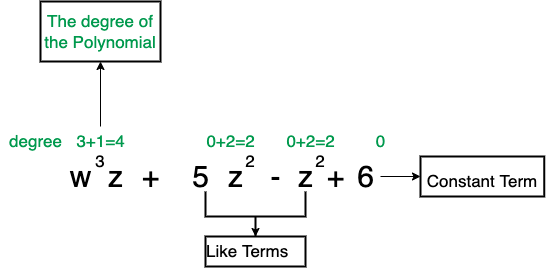
\includegraphics[width=0.8\linewidth]{Polynomial.png}
			\end{figure}
			\begin{itemize}
				\item Like Terms\ 同类项
				\item The Degree of a Polynomial\ 多项式的次数
			\end{itemize}
\end{frame}

%------------------------------------------------

\begin{frame}
	\frametitle{A Real QR Problem!}
	\framesubtitle{}
	\begin{figure}
		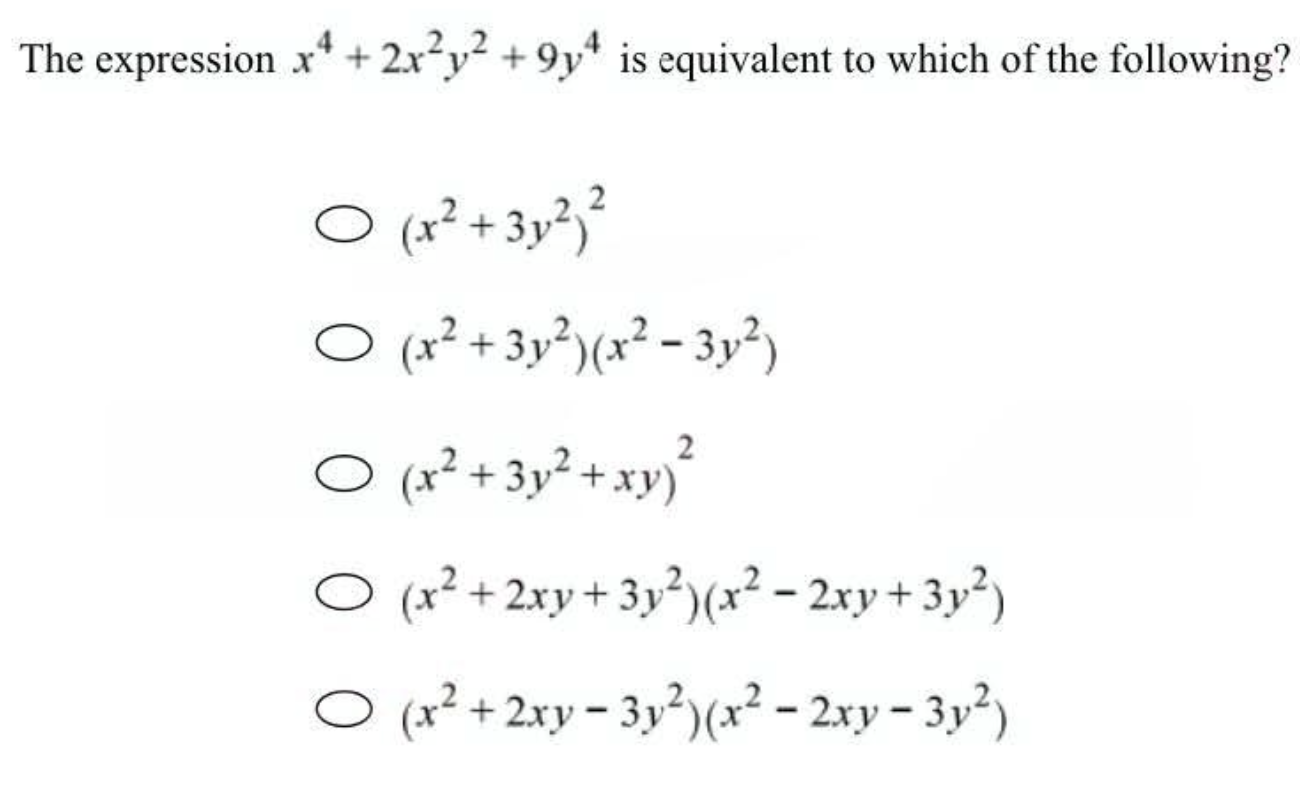
\includegraphics[width=0.7\linewidth]{Algebra_Expression_Example_Question1.png}
		\caption{10-Sec3-19}
	\end{figure}
	\pause
 凑中间项的系数
\pause
\bigskip
Answer \textbf{D } 
\end{frame}

\section{Coordinate Geometry}
% Coordinates scale
\begin{frame}
	\frametitle{To Begin With}
	\begin{block}{QR Mathematical Convention 2 }
		When coordinate systems, such as and number lines, are
shown with scales, you should read, estimate, or compare quantities by
sight or by measurement, \alert{according to the corresponding scales}.
	\end{block}
\end{frame}
%------------------------------------------------

%------------------------------------------------



\begin{frame}
	\frametitle{Terminologies of Coordinate Geometry}
	\framesubtitle{坐标系专业名词}
	{\LARGE 象限的英文怎么说?}
	\pause
	\begin{figure}
		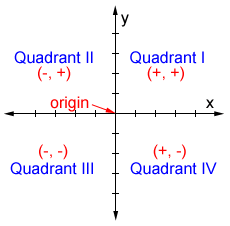
\includegraphics[width=0.5\linewidth]{Signs_Of_Quadrant.png}
	\end{figure}
\end{frame}

%------------------------------------------------

 \section{Linear Problems}

%------------------------------------------------

\subsection{Linear Function}

%------------------------------------------------

\begin{frame}
	\frametitle{Slope and Intercepts}
	\framesubtitle{斜率和截距}

	\begin{columns}[t] 
		\begin{column}{0.4\textwidth} % Left column width
			\begin{definition}
						The graph of a linear equation of the form $y = mx + b$ is a straight line
				in the $xy-plane$, where m is called the \alert{slope} of the line and b is called the \alert{y-intercept}. \\
				The x-intercepts of a graph are the \alert{x-coordinates} of the points at which the graph intersects the x-axis.
			\end{definition}
		\end{column}
		\begin{column}{0.6\textwidth} % Right column width
			\begin{figure}
				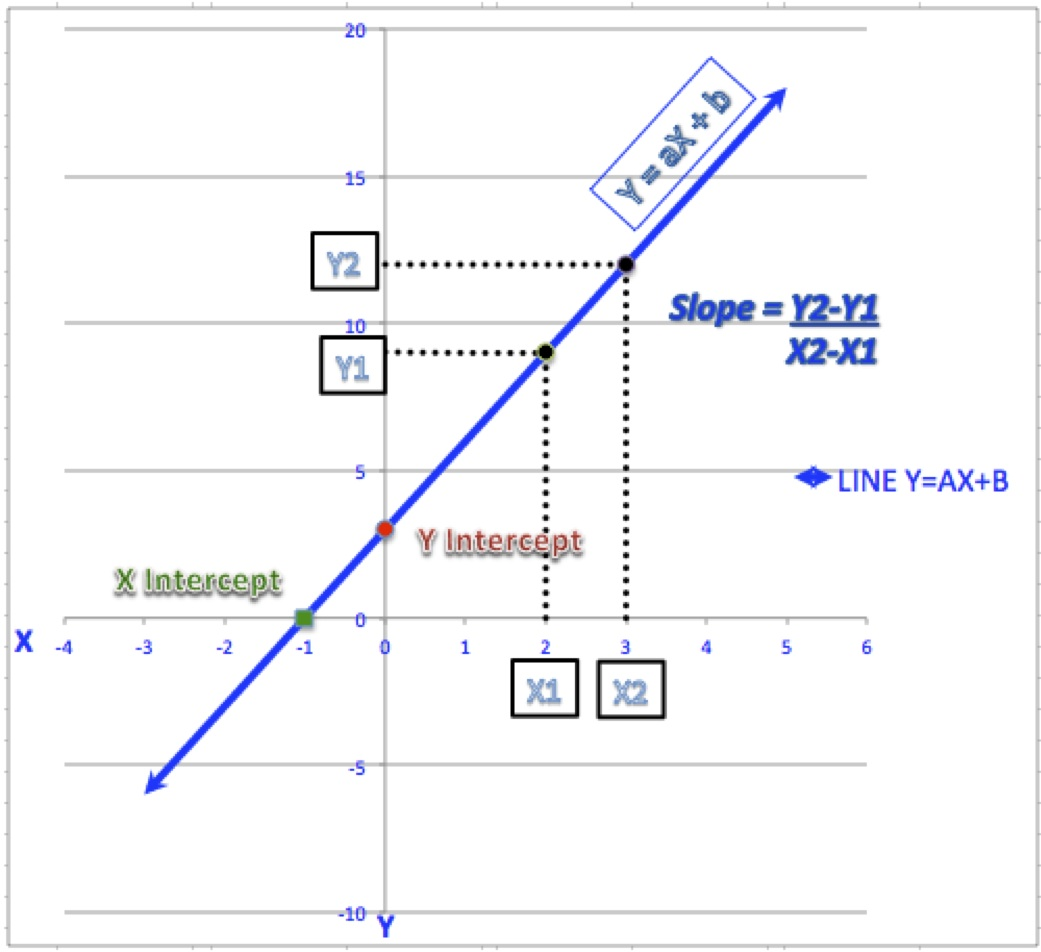
\includegraphics[width=\linewidth]{how-to-calculate-slope-and-intercepts-of-a-line-thumb-mMPHze60u.jpeg}
			\end{figure}
    \end{column}
	\end{columns}
\end{frame}

%------------------------------------------------

\begin{frame}
	\frametitle{Have a try!}
	\framesubtitle{两点确定一条直线}
	\textbf{og-p385-2.8.1}
	Below shows the graph of the line through the points Q(−2, −3) and R(4, 1.5).

	\begin{columns}[t] 
		\begin{column}{0.6\textwidth} % Left column width
			\begin{figure}
		    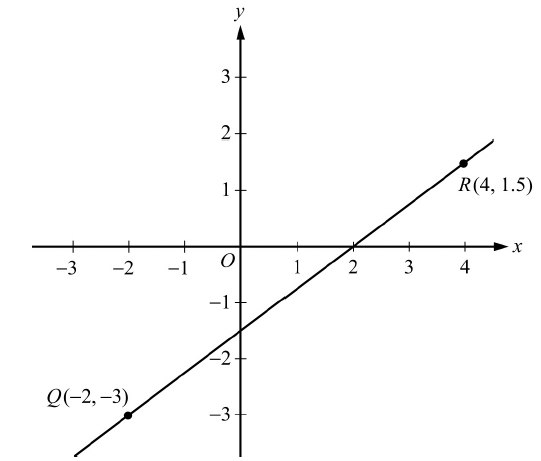
\includegraphics[width=\linewidth]{Linear_Function_Example_Question_1.png}
	   \end{figure}
		\end{column}
		\begin{column}{0.4\textwidth} % Right column width
		\pause
		$y = 0.75x - 1.5$ \\ 看图 Drawn to scale \\
		\bigskip
		$slope = \frac{1.5 -(-3) }{4- (-2)} = \frac{4.5}{6} = \frac{3}{4} = 0.75$ \\
		$y-intercept= (-3) - 0.75  \times (-2) = -1.5$\\
    \end{column}
	\end{columns}
\end{frame}

%------------------------------------------------

\begin{frame}
	\frametitle{A Real QR Problem!}
	\framesubtitle{}
	\begin{figure}
		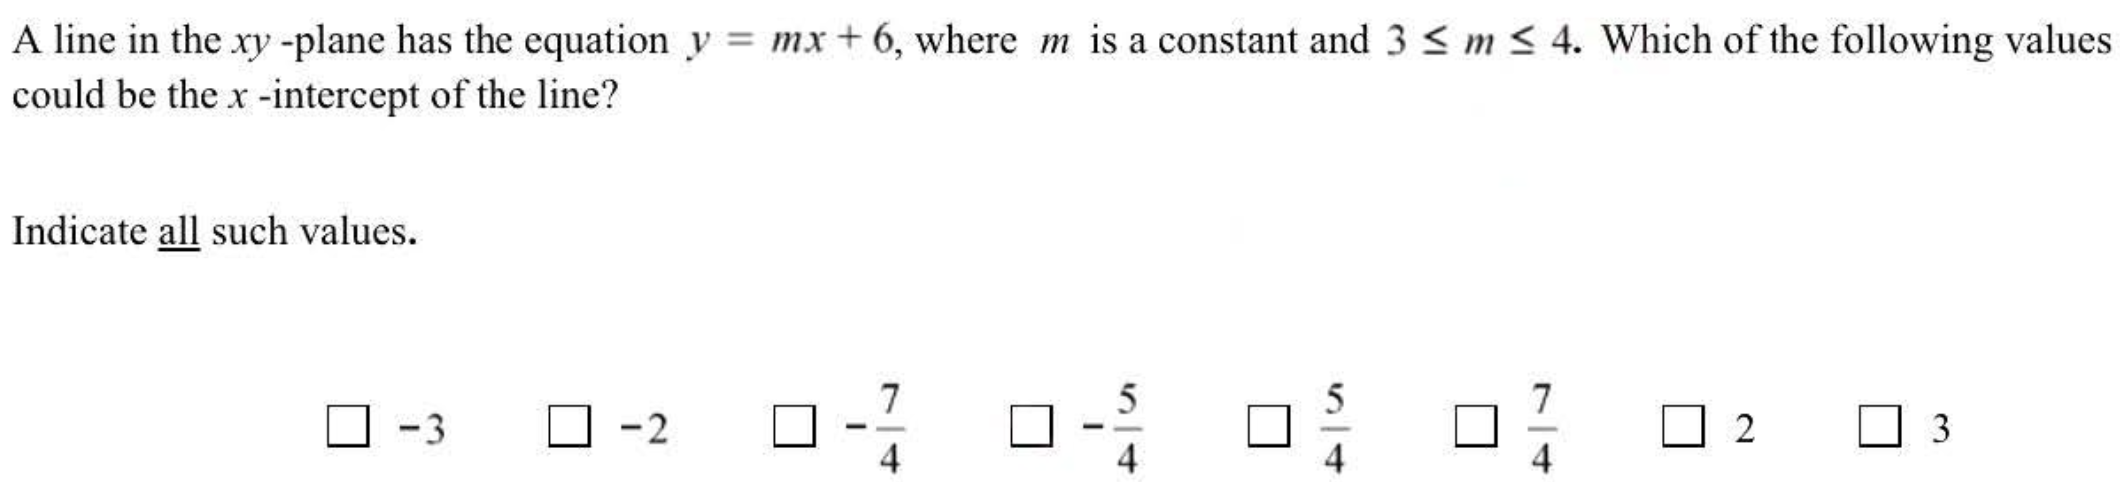
\includegraphics[width=\linewidth]{Graphing_Linear_Equations_Example_Question1.png}
		\caption{6-Sec3-18}
	\end{figure}

	\begin{columns}[t] 
		\begin{column}{0.45\textwidth} % Left column width
			\pause
			$-2\leq x \leq -1.5$\\
			\pause
			\bigskip
			Answer \textbf{BC} $-2;-\frac{7}{4}$ 
		\end{column}
		\begin{column}{0.5\textwidth} % Right column width
			\begin{figure}
				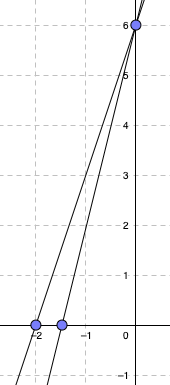
\includegraphics[width=0.2\linewidth]{Graphing_Linear_Equations_Example_Question1_1.png}
			\end{figure}
    \end{column}
	\end{columns}
\end{frame}

%------------------------------------------------


\begin{frame}
	\frametitle{A Real QR Problem!}
	\framesubtitle{}
	\begin{figure}
		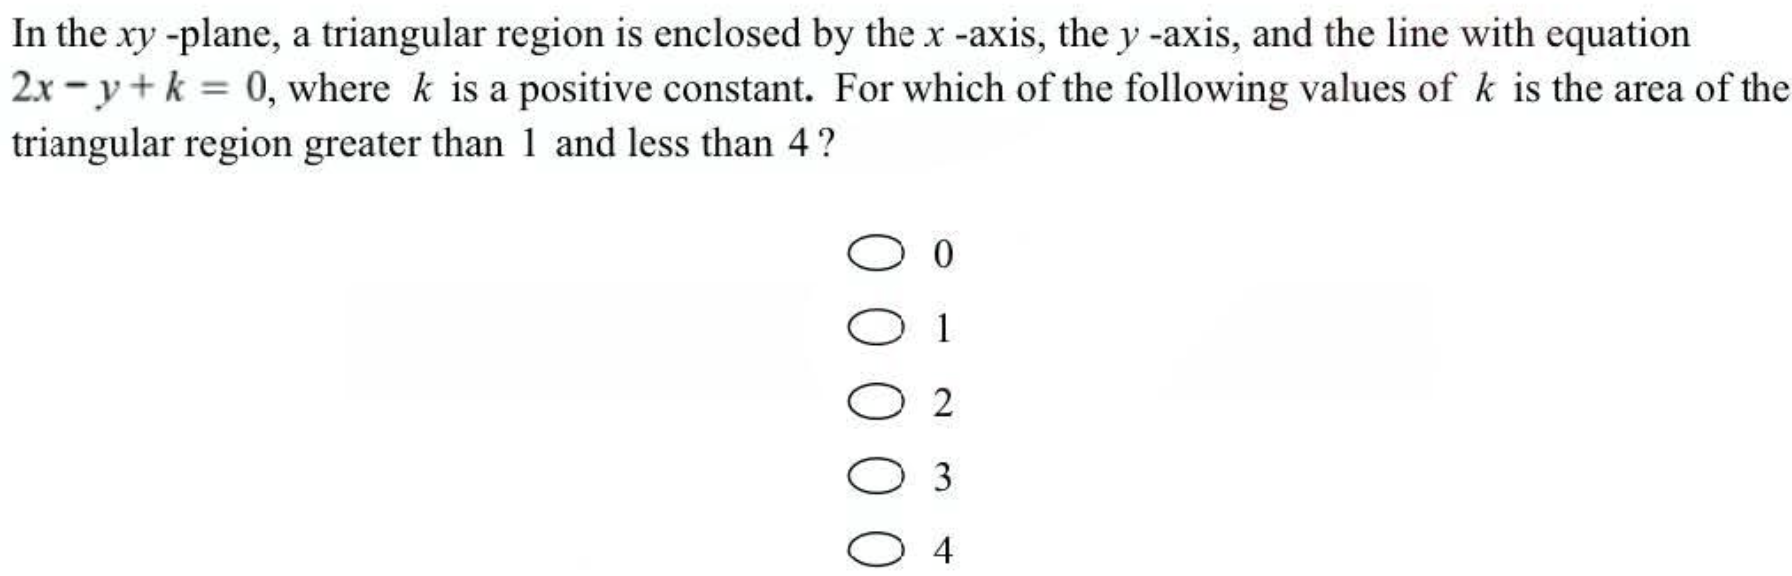
\includegraphics[width=\linewidth]{Graphing_Linear_Equations_Example_Question2.png}
		\caption{9-Sec2-10}
	\end{figure}

	\begin{columns}[t] 
		\begin{column}{0.45\textwidth} % Left column width
			\pause
			$4\leq k \leq 2$\\
			\pause
			\bigskip
			Answer \textbf{D} $k=3$ 
		\end{column}
		\begin{column}{0.2\textwidth} % Right column width
			\begin{figure}
				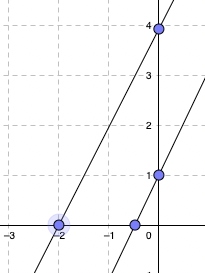
\includegraphics[width=0.5\linewidth]{Graphing_Linear_Equations_Example_Question2_1.png}
			\end{figure}
    \end{column}
	\end{columns}
\end{frame}

%------------------------------------------------

\begin{frame}
	\frametitle{The Relation of Slopes for Parallel or Perpendicular }
	\framesubtitle{平行或垂直直线斜率关系}

	\begin{columns}[t] 
		\begin{column}{0.5\textwidth} % Left column width

			\begin{figure}
		    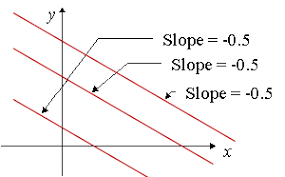
\includegraphics[width=\linewidth]{Parallel_Slopes.png}
		    \caption{Two lines are parallel if their slopes are equal.}
	   \end{figure}
		\end{column}

		\begin{column}{0.5\textwidth} % Right column width
			\begin{figure}
		    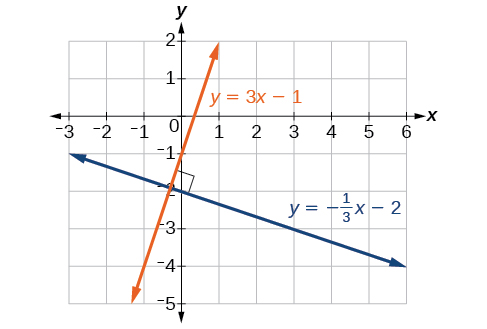
\includegraphics[width=\linewidth]{Perpendicular_Slopes.jpeg}
		    \caption{Two lines are perpendicular if their slopes are negative reciprocals of each other.}
	   \end{figure}
    \end{column}
	\end{columns}
\end{frame}

%------------------------------------------------

\begin{frame}
	\frametitle{A Real QR Problem!}


	\begin{figure}
		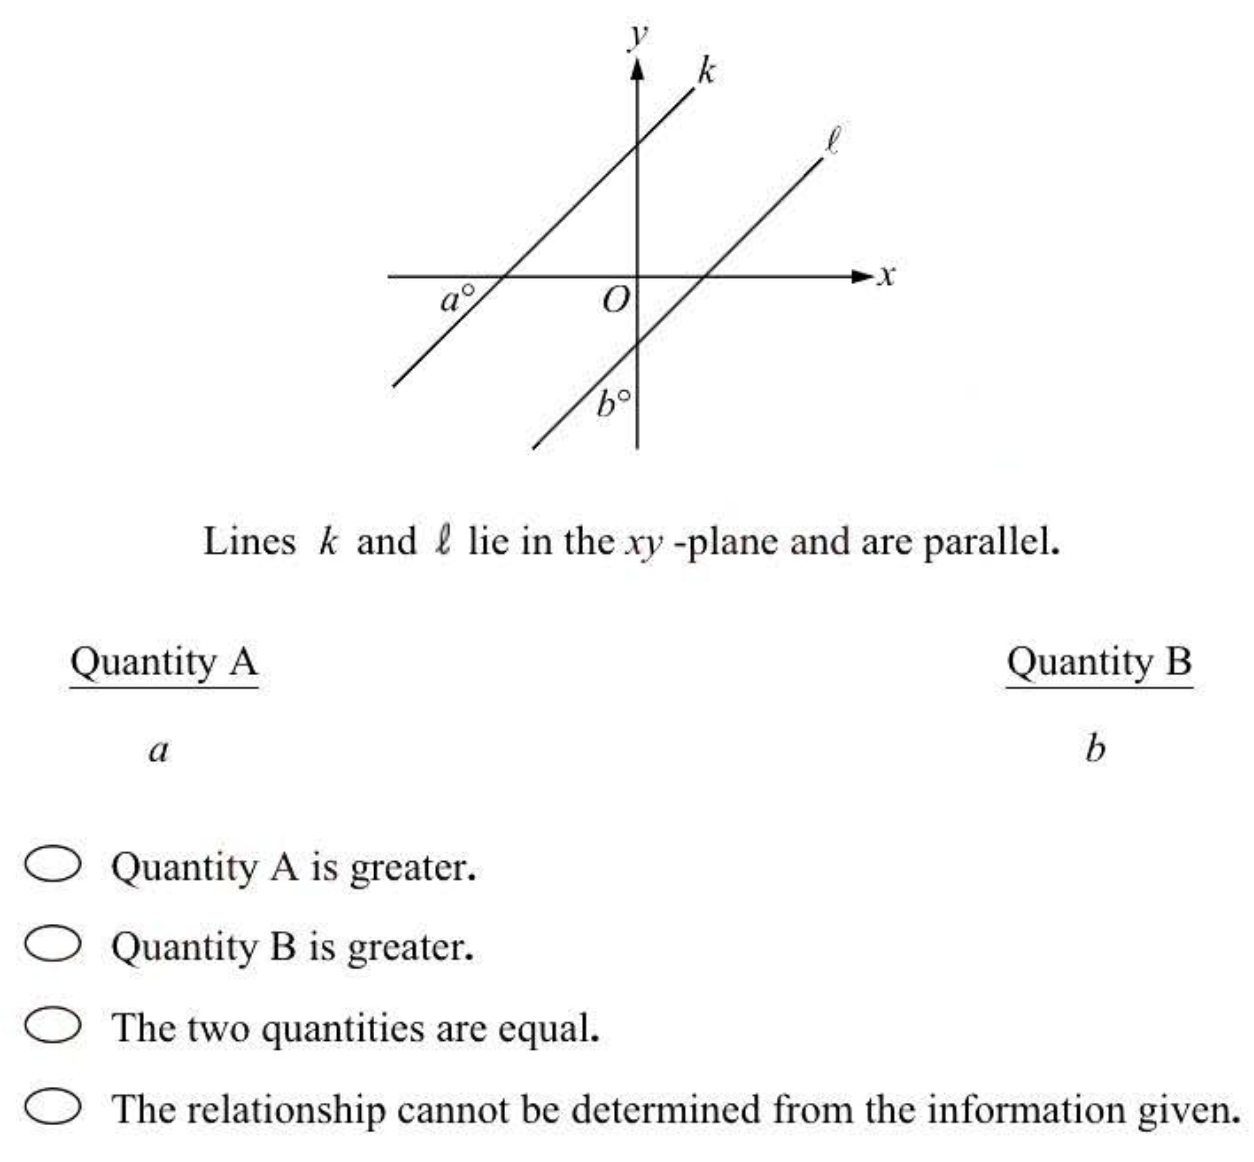
\includegraphics[width=0.5\linewidth]{Parallel_Slopes_Example_Question1.png}
		\caption{6-Sec3-7}
	\end{figure}
	\pause
a  \textdegree+ b  \textdegree= 90 \textdegree   \\
\pause
\bigskip
Answer \textbf{D } The relationship cannot be determined from the information given.
\end{frame}

%------------------------------------------------


\begin{frame}
	\frametitle{Calculating the Distance Between Two Points}
	\framesubtitle{两点间距离}
	\begin{columns}[t] 
		\begin{column}{0.6\textwidth} % Left column width
			\begin{figure}
		    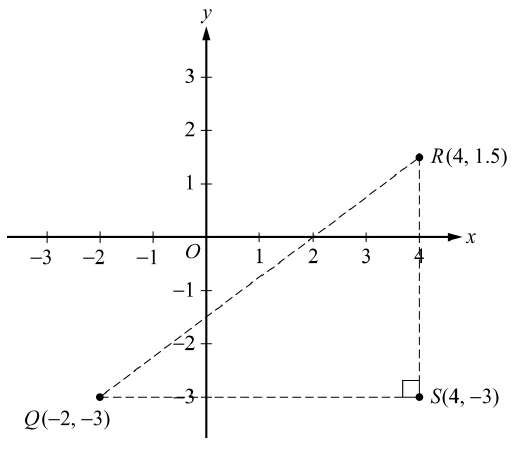
\includegraphics[width=\linewidth]{Distance_Between _Two_Points.png}
		 \end{figure}
		\end{column}
		\begin{column}{0.4 \textwidth} % Right column width
			\begin{equation*}
				\begin{aligned}
				&QR\\
				&= \sqrt{QS^2 + RS^2}\\
				&= \sqrt{(x_1 - x_2)^2 + (y_1 - y_2)^2}\\
				&= \sqrt{6^2 + 4.5^2}\\
				&= 7\\
				\end{aligned}
			\end{equation*}

    \end{column}
	\end{columns}
\end{frame}

%------------------------------------------------


\subsection{Linear Equations in One Variable}

%------------------------------------------------

\begin{frame}
	\frametitle{Equivalent Equations}
	\framesubtitle{等价方程}
	\begin{definition}
		Two equations that have the \alert{same} solutions are called equivalent equations.
	\end{definition}
	
	\smallskip % Vertical whitespace
	
	\begin{example}

  $x + 1 = 2$ and $2x + 2 = 4$

	\end{example}
	\end{frame}

%------------------------------------------------	
\subsection{Linear Equations in Two Variable}

%------------------------------------------------	

	\begin{frame}
	\frametitle{Solution For Linear Equations in Two Variables}
	\framesubtitle{交点就是Solution}
	\begin{columns}[t] 
		\begin{column}{0.3\textwidth} % Left column width
		\begin{equation*}
			\begin{aligned}
				4x + 3y &= 13 \\
				x + 2y &= 2
			\end{aligned}
		\end{equation*}

		\bigskip
		\begin{equation*}
			\begin{aligned}
				y &= -\frac{3}{4} + \frac{13}{4} \\
				y &= -\frac{1}{2}x + 1
			\end{aligned}
		\end{equation*}

		\end{column}
		\begin{column}{0.7\textwidth} % Right column width
			\begin{figure}
				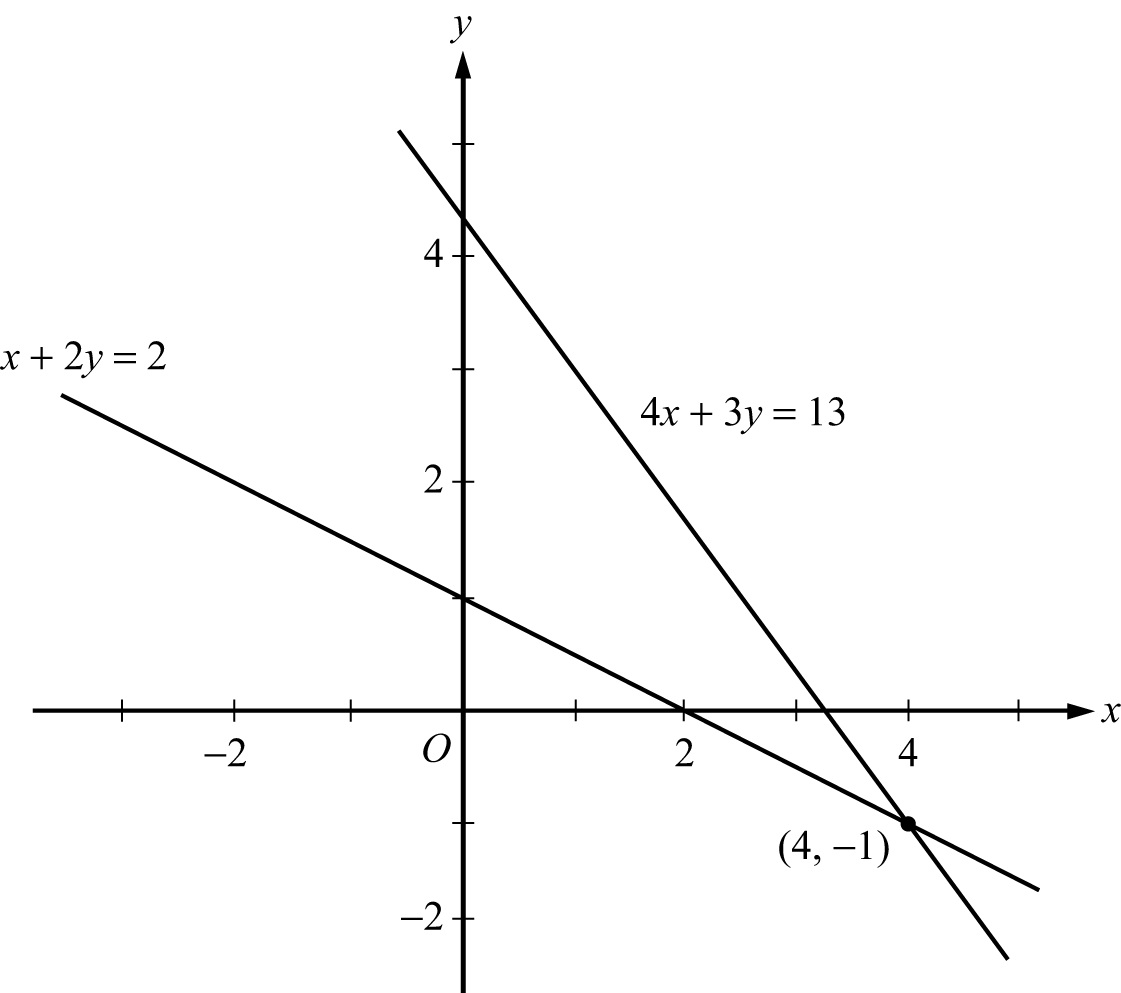
\includegraphics[width=0.8\linewidth]{Graphing_Linear_Equations.jpg} 
			\end{figure}
    \end{column}
	\end{columns}	
\end{frame}
%------------------------------------------------

\subsection{Solving Linear Inequalities}

%------------------------------------------------

\begin{frame}
	\frametitle{Solution Set}
	\framesubtitle{线性不等式的解集}
	\begin{definition}
			To solve an inequality means to find the set of all values of the variable that make the inequality true. This set of values is also known as the \alert{solution set} of an inequality.
	\end{definition}
	
	\smallskip % Vertical whitespace
		
	\begin{figure}
		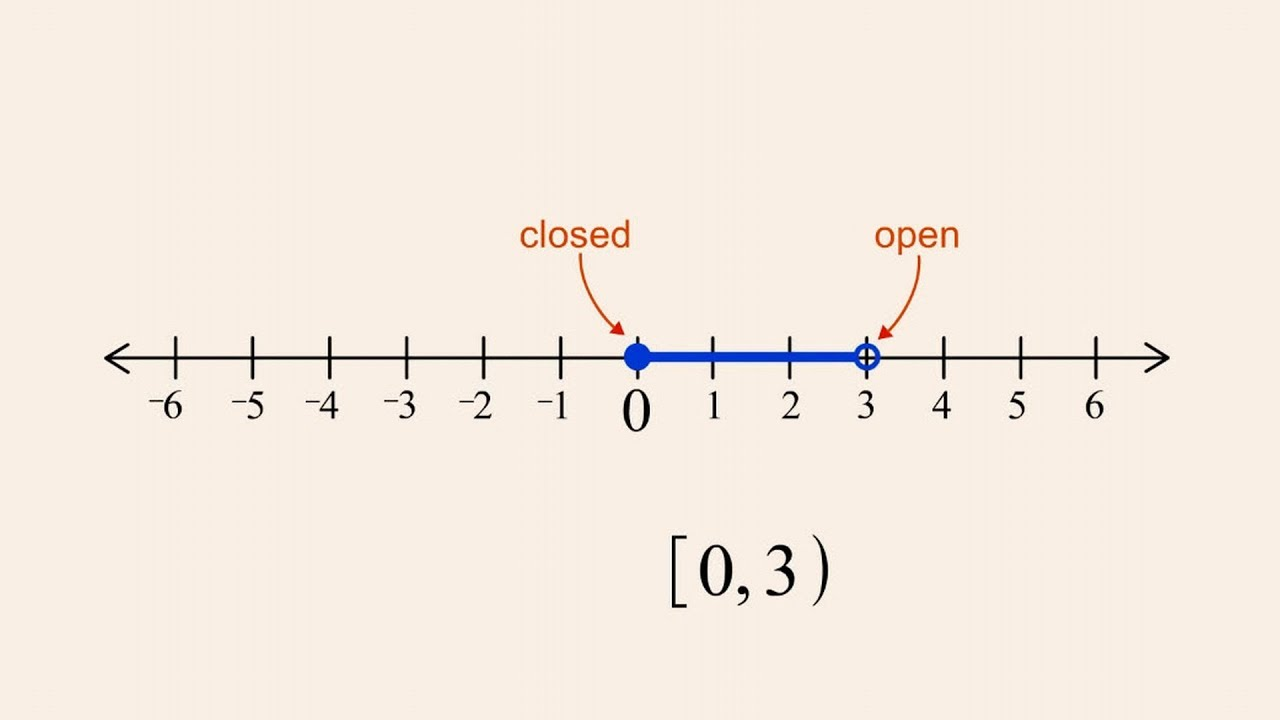
\includegraphics[width=0.8\linewidth]{Solution_Set.jpeg}
	\end{figure}

\end{frame}
%------------------------------------------------

\begin{frame}
	\frametitle{Equivalent Inequalities}
	\framesubtitle{等价不等式}
	\begin{definition}
		Two inequalities that have the \alert{same} solution set are called equivalent inequalities.
	\end{definition}
	
	\smallskip % Vertical whitespace
	
	\begin{example}
  $-3x +5 \leq 17 $ and $-3x \leq 12$
	\end{example}
	\end{frame}
	
%------------------------------------------------

\begin{frame}
	\frametitle{The Big Question }
	{\LARGE How to we find Equivalent Inequalities}

\end{frame}

%------------------------------------------------

\begin{frame}
	\frametitle{Addition and Subtraction in  Linear Inequalities}
	\framesubtitle{不等式两边同加减一个数,不等式仍成立}

	\begin{theorem}[Rule 1]
		When the same constant is added to or subtracted from both sides of an inequality, the direction of the inequality is preserved and the new inequality is equivalent to the original.
	\end{theorem}

	\begin{example}
		\begin{itemize}
			\item   $-3x +5 \leq 17 $ and $-3x \leq 12$
			\item   $72x  \geq 81 $ and $72x  -81 \geq 0 $
		\end{itemize}
	\end{example}

\end{frame}

%------------------------------------------------



\begin{frame}
	\frametitle{Multiplying or Dividing in  Linear Inequalities}
	\framesubtitle{正同负反}
	\begin{theorem}[Rule 2]
		When both sides of the inequality are multiplied or divided by the same nonzero constant, the direction of the inequality is \alert{preserved if the constant is positive} but the direction is \alert{reversed if the constant is negative}.
	\end{theorem}

	\begin{example}
	  \begin{equation*}
	  	\begin{split}
	  		-3x + 15 &\leq 17\\
	  		-3x &\leq 12 \\
	  		3x &>12 \\
	  		x &> 4\\
	  	\end{split}
	  \end{equation*}
	\end{example}
\alert{负号就是关于原点对称}
\end{frame}

%------------------------------------------------

\subsection{Linear Inequalities In Two Variable}

%------------------------------------------------

	\begin{frame}
	\frametitle{Solution Set For Linear Inequalities in Two Variables}
	\framesubtitle{}
	\begin{columns}[t] 
		\begin{column}{0.3\textwidth} % Left column width
		\begin{equation*}
			\begin{aligned}
				x - 3y &\geq -6 \\
				2x + y &=\geq -1
			\end{aligned}
		\end{equation*}

		\bigskip
		\begin{equation*}
			\begin{aligned}
				y &\leq \frac{1}{3} + 2\\
				y &\geq -2x + 1
			\end{aligned}
		\end{equation*}

		\end{column}
		\begin{column}{0.7\textwidth} % Right column width
			\begin{figure}
				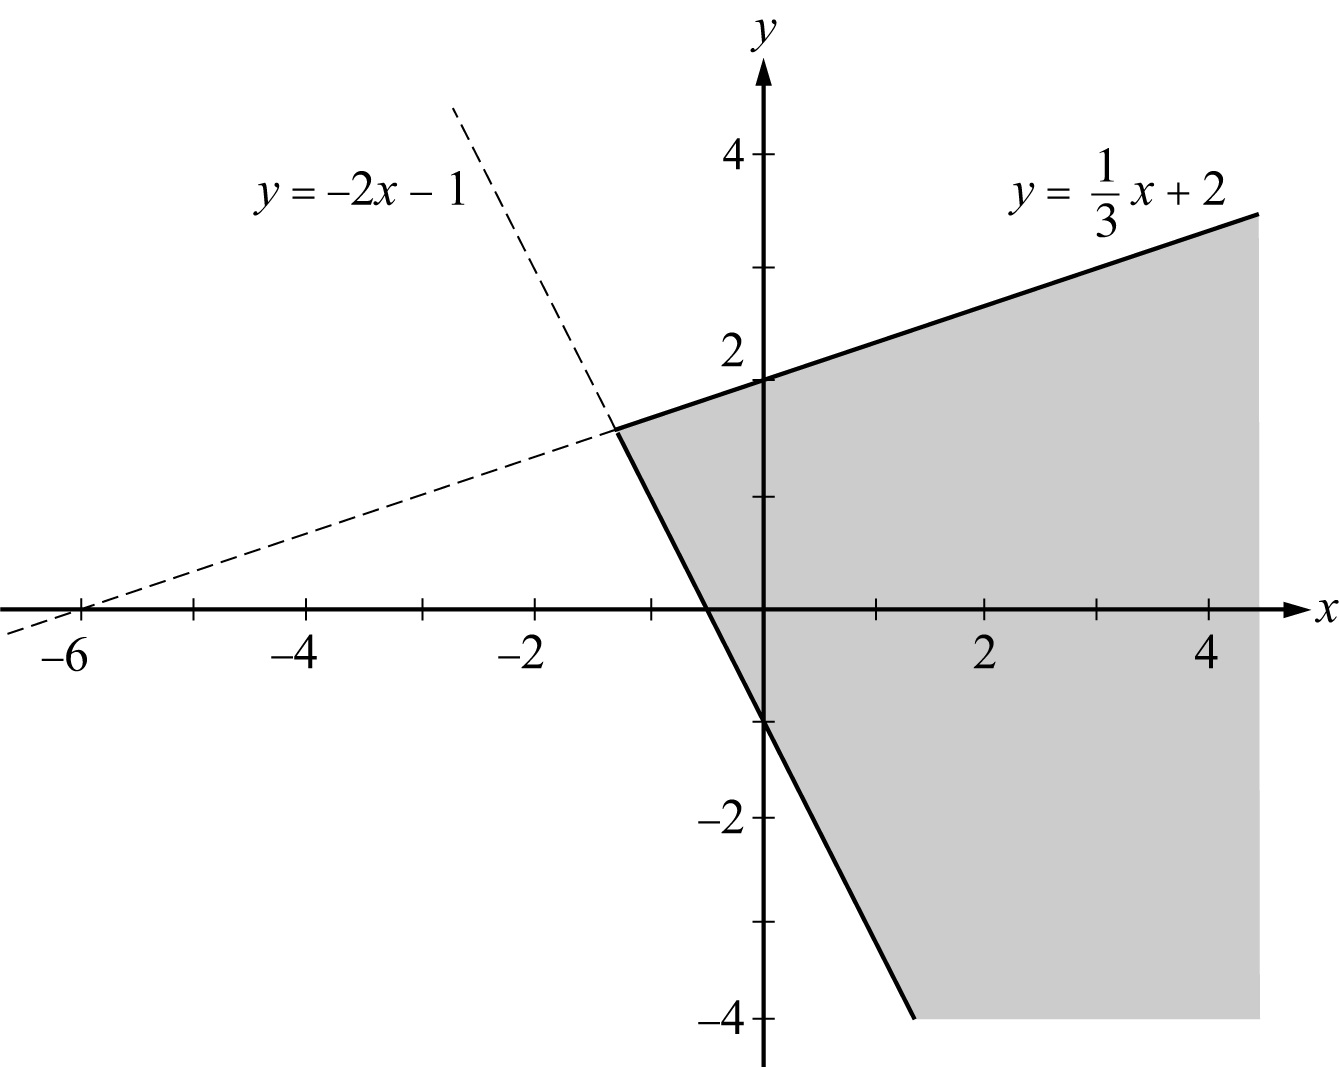
\includegraphics[width=0.8\linewidth]{Linear_Inequalities_In_Two_Variable.jpg} 
			\end{figure}
    \end{column}
	\end{columns}	
\end{frame}
%------------------------------------------------


%------------------------------------------------

\section{Quadratic Problems}

%------------------------------------------------

\subsection{Quadratic Function}

%------------------------------------------------


\begin{frame}
	\frametitle{The Opening and Vertex of a Parabola}
	\framesubtitle{抛物线开口和顶点}
			\begin{definition}
		The graph of a quadratic equation of the form $y = ax^2 + bx +c $, where a, b, and c are constants and $a\neq 0$ , is a \alert{parabola}. The symmetric axis is  $x= -\frac{b}{2a}$
			\end{definition}

			\begin{figure}
				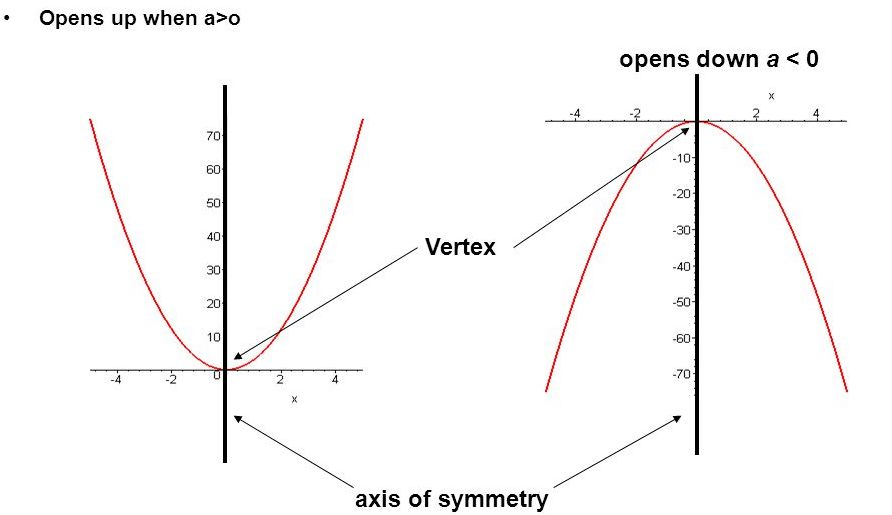
\includegraphics[width=0.6\linewidth]{Parabola.jpeg}
			\end{figure}

\end{frame}

%------------------------------------------------

\begin{frame}
	\frametitle{A Real QR Problem!}
	\framesubtitle{}

	\begin{figure}
		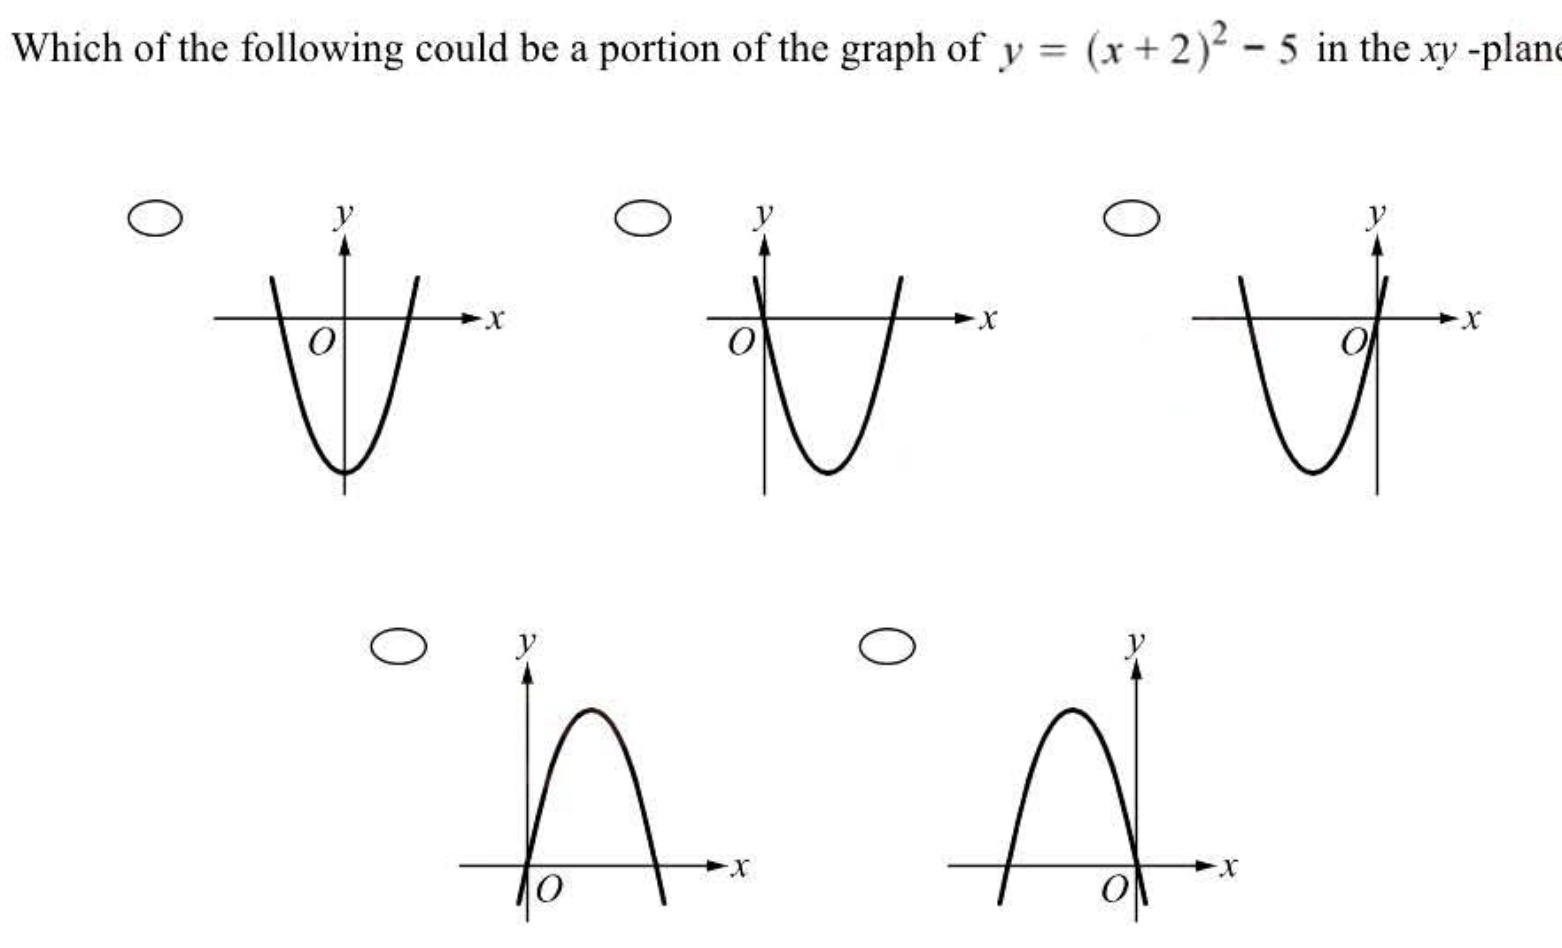
\includegraphics[width=0.7\linewidth]{Parabola_Example_Question1.png}
		\caption{6-Sec3-11}
	\end{figure}

	\pause

看开口,看对称轴,看y-intercept,看vertex的坐标 \\

\pause

\bigskip
Answer \textbf{C } \pause Please state the signs of a and b for other graphs.

\end{frame}

%------------------------------------------------

\begin{frame}
	\frametitle{Have a try!}
	\framesubtitle{}

In the range of $-3/4 < x < -1/2$, what is the least possible value of x?
\bigskip
	\begin{columns}[t] 
		\begin{column}{0.45\textwidth} % Left column width
			\begin{enumerate}[A]
				\item $x$
				\item $x + 3$
				\item $x^2 -3x$
				\item $x^3 - x$
				\item $x^4$
			\end{enumerate}
		\end{column}
		\begin{column}{0.5\textwidth} % Right column width
		  \pause
			\begin{enumerate}[A]
				\item $x <0$ 
				\item $x + 3 >0$ 
				\item $x^2 -3x>0$ since $x=\frac{4}{3}$ is the symmetric axis and the opening is upward
				\item $x^3 - x= x(x^2 - 1) >0$ since $x^2 <1$
				\item $x^4>0$
			\end{enumerate}
		\bigskip
    Answer \textbf{A}
    \end{column}
	\end{columns}
\end{frame}

%------------------------------------------------

\subsection{Solving Quadratic Equations By the Quadratic Formula Or Factoring}

%------------------------------------------------


\begin{frame}
	\frametitle{Solving Quadratic Equations}
	\framesubtitle{一元二次方程公式\ 因式分解}

	\begin{columns}[t] 
		\begin{column}{0.5\textwidth} % Left column width
				\begin{theorem}[一元二次方程公式]
					For $y = ax^2 + bx + c$, the solutions is \\
					\begin{equation*}
						x=\frac{-b \pm \sqrt{b^2 - 4ac}}{2a}
					\end{equation*}
				\end{theorem}

				\begin{example}
					\begin{equation*}
						\begin{aligned}
							&2x^2 -x - 6 = 0 \\
							&x = \frac{-(-1) \pm \sqrt{(-1)^2 - 4(2)(-6)}}{2(2)} \\
							&= \frac{1 \pm 7}{4} = 2\ or\ -\frac{3}{2} 
						\end{aligned}
					\end{equation*}
				\end{example}
		\end{column}
		\begin{column}{0.45\textwidth} % Right column width
				\textbf{因式分解(配方法}

				\begin{example}
					\begin{equation*}
						\begin{aligned}
							&2x^2 -x - 6 = 0 \\
							&2(x^2 - 2 \cdot \frac{1}{4}x +  \frac{1}{16})-\frac{49}{8} = 0 \\
							&2(x - \frac{1}{4})^2-\frac{49}{8} = 0 \\
							&(x - \frac{1}{4})^2=\frac{49}{16} \\
							& x - \frac{1}{4}=\pm \frac{7}{4} \\
							&x = 2 \ or \ -\frac{3}{2}
						\end{aligned}
					\end{equation*}
				\end{example}
    \end{column}
	\end{columns}
\end{frame}

%------------------------------------------------

\begin{frame}
	\frametitle{Have a try!}
	\framesubtitle{Parabola和X轴交点就是Solution}
   \textbf{og-p390-2.8.5} Consider the line whose equation is $y = x^2 - 2x - 3$. Find the solution when $y = 0$.
	\begin{columns}[t] 
		\begin{column}{0.4\textwidth} % Left column width
		\pause
		$(x- 3)(x+ 1) = 0$\\
		\bigskip
    Answer \textbf{$x  = -1 \ or \ 3 $}
		\end{column}
		\begin{column}{0.6\textwidth} % Right column width
		  \begin{figure}
				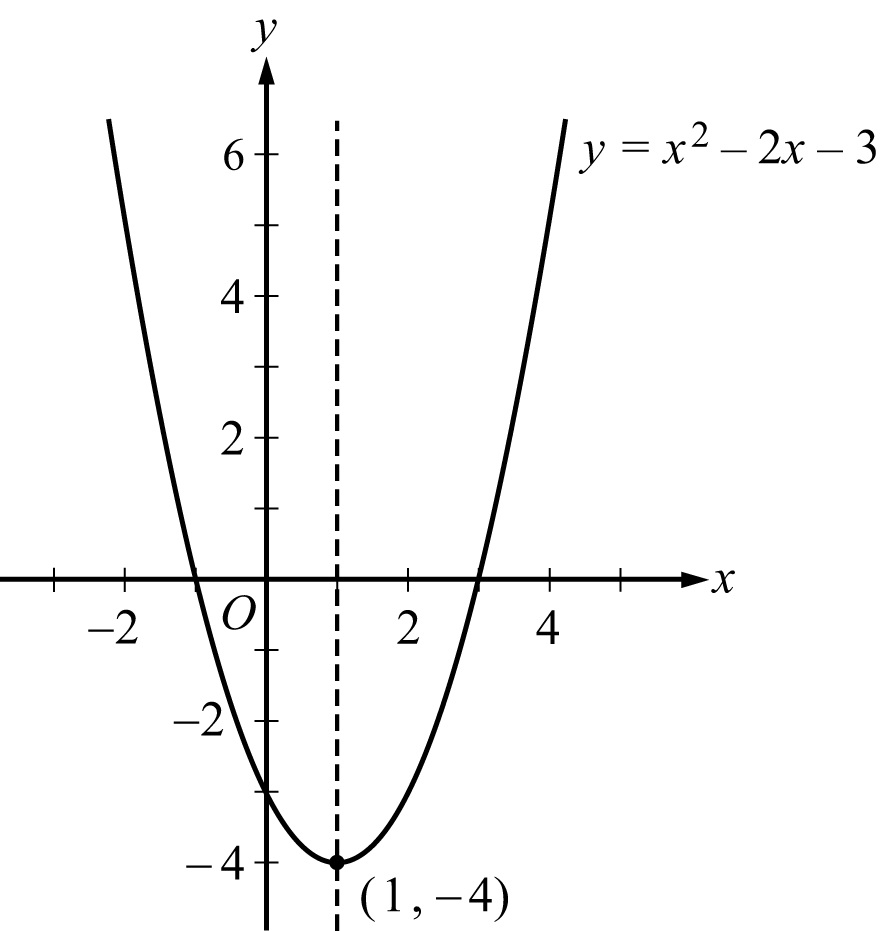
\includegraphics[width=0.6\linewidth]{Graphing_Quadratic_Equations.jpg} 
			\end{figure}
    \end{column}
	\end{columns}
\end{frame}

%------------------------------------------------

%------------------------------------------------

\subsection{Graphing Circles}

%------------------------------------------------

\begin{frame}
	\frametitle{Circles}
	\framesubtitle{到定点距离都相等}
	\begin{theorem}[圆]
		$(x - a)^2 + (y - b)^2 = r^2$ is a circle with its center at the point $(a, b)$ and with radius $r >0$.
	\end{theorem}

		\begin{figure}
		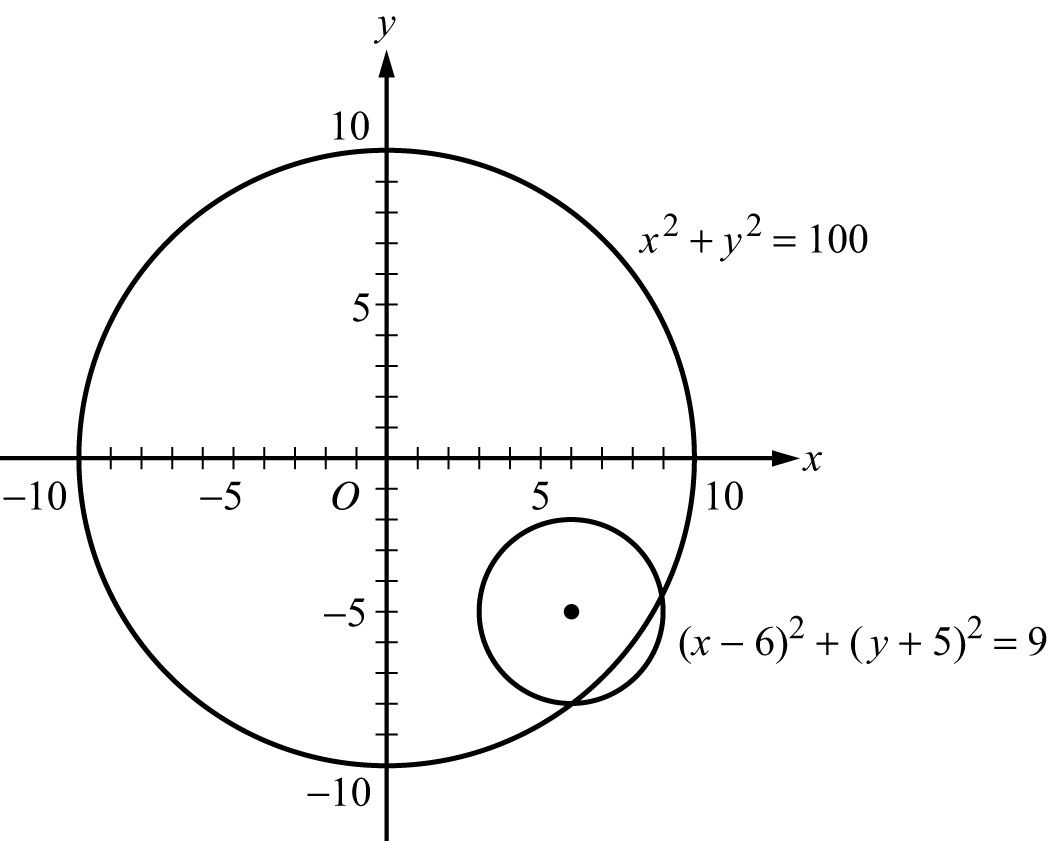
\includegraphics[width=0.6\linewidth]{Circles.jpg}
	\end{figure}
\end{frame}

%------------------------------------------------

%------------------------------------------------

\section{Piecewise-Defined Function}

%------------------------------------------------


\begin{frame}
	\frametitle{Piecewise-Defined Function}
	\framesubtitle{}

\[y= \begin{cases} 
      -x & x\leq 0 \\
      x &  x\geq 0 \\
   \end{cases}
\]
	\begin{figure}
		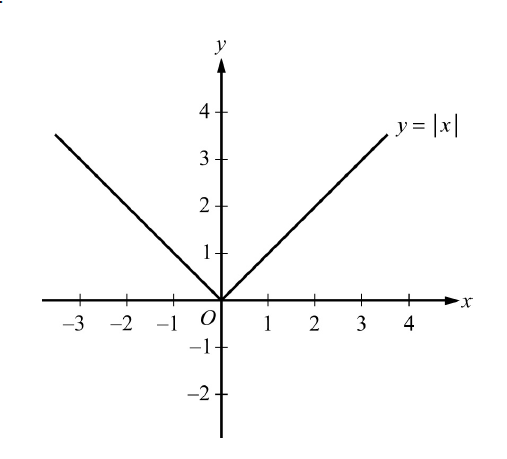
\includegraphics[width=0.5\linewidth]{Piecewise_Defined_Function.png}
		\caption{$y = \mid x \mid$}
	\end{figure}

\end{frame}

\section{Reflecting, Shifting and Stretching of Functions}

%------------------------------------------------
\subsection{Reflecting Functions}
\begin{frame}
	\frametitle{Reflecting Functions about $y = x$}
	\begin{theorem}[关于$y=x$镜像对称:调换xy]
	The inverse funtions are the reflection of each other about $y = x$
	\end{theorem}

	\begin{figure}
		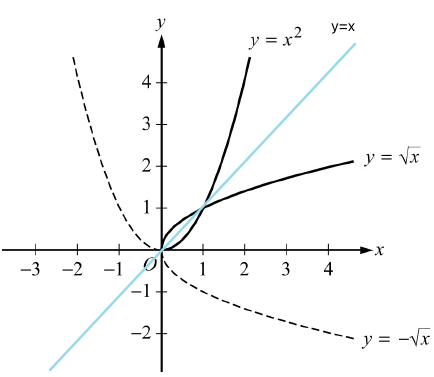
\includegraphics[width=0.5\linewidth]{Reflection1.png} 
	\end{figure}
\end{frame}

%------------------------------------------------

\begin{frame}
	\frametitle{Have a try!}
	\framesubtitle{x 和 y 对调}
   \textbf{og-p390-2.8.4} Consider the line whose equation is $y = 2x + 5$. Find the equation that is reflection of $y = 2x + 5$ about $y=x$.
	\begin{columns}[t] 
		\begin{column}{0.4\textwidth} % Left column width
		\pause
		$x = 2y + 5$\\
		\bigskip
    Answer \textbf{$y  = \frac{1}{2} x - \frac{5}{2}$}
		\end{column}
		\begin{column}{0.6\textwidth} % Right column width
		  \begin{figure}
				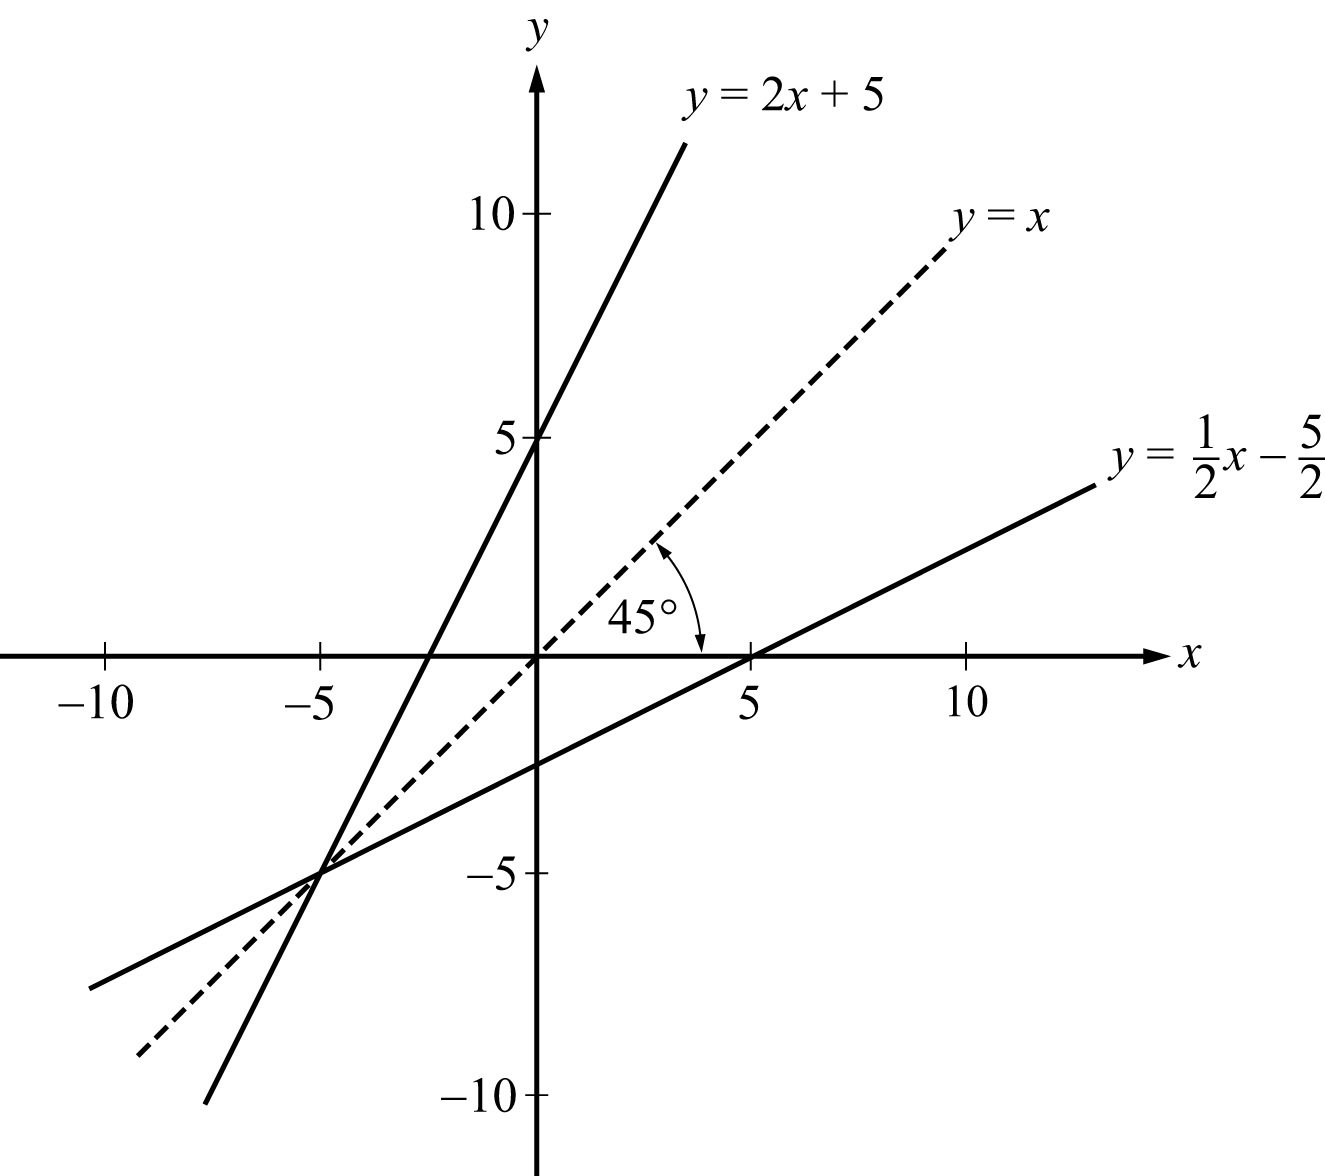
\includegraphics[width=\linewidth]{Reflection3.jpg} 
			\end{figure}
    \end{column}
	\end{columns}
\end{frame}

%------------------------------------------------

\begin{frame}
	\frametitle{Reflecting Functions about $x-axis$}
	\begin{theorem}[关于x轴镜像对称:函数右边加负号]
	In general, for any function h, the graph of $y = −h(x)$ is the reflection of the graph of $y = h(x)$ about the x-axis.
	\end{theorem}
	\begin{figure}
		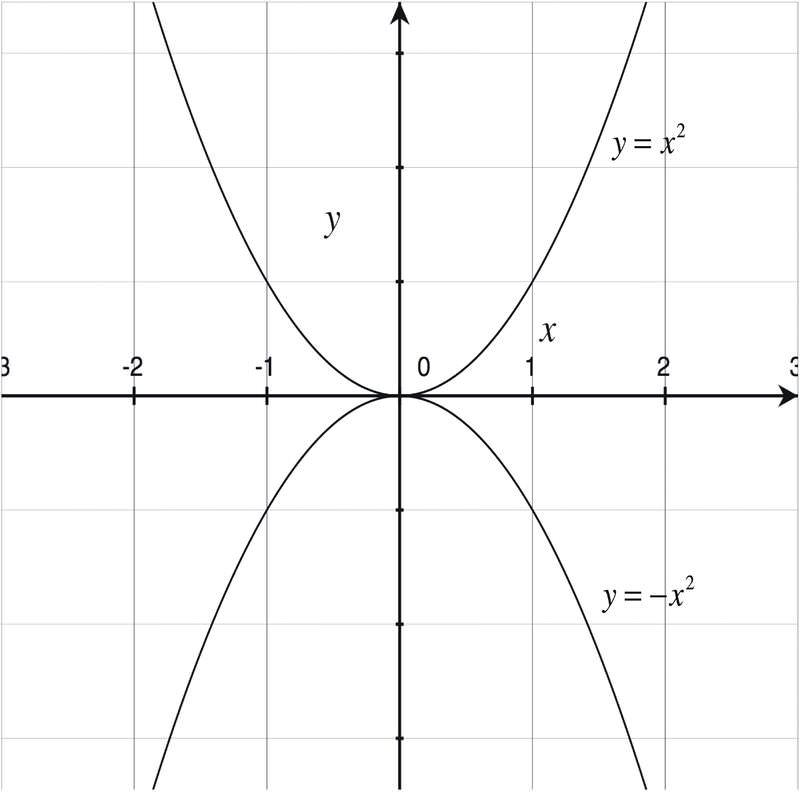
\includegraphics[width=0.5\linewidth]{Reflection2.jpeg} 
	\end{figure}
\end{frame}

%------------------------------------------------

\subsection{Shifting Functions}
\begin{frame}
	\frametitle{Shifting Functions Upward or Downward}
	\begin{theorem}[上下平移:函数右边加常数项]
		\begin{itemize}
			\item The graph of $h(x) + c$ is the graph of $h(x)$ shifted upward by c units. 
			\item The graph of $h(x) - c$ is the graph of $h(x)$ shifted downward by c units.
		\end{itemize}
	\end{theorem}
	

	\begin{figure}
		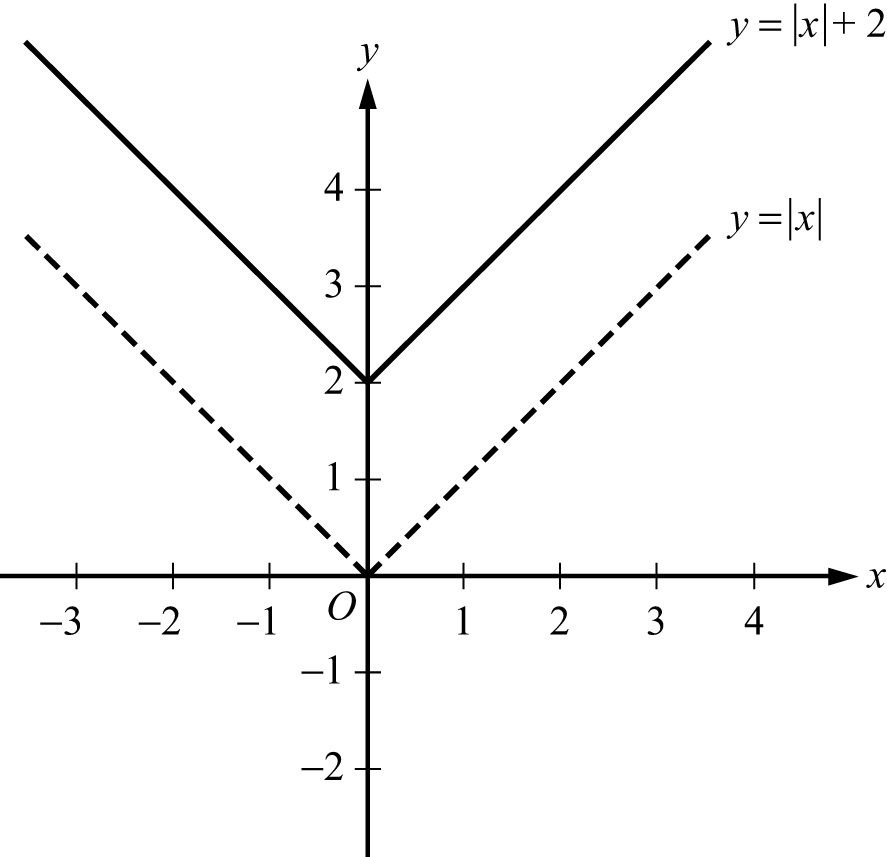
\includegraphics[width=0.5\linewidth]{Shifting_Function1.jpg} 
	\end{figure}

\end{frame}

%------------------------------------------------

\begin{frame}
	\frametitle{Shifting Functions to the Left or Right}
	\begin{theorem}[左右平移:在x上加减]
		\begin{itemize}
			\item The graph of $h(x+c) $is the graph of $h(x)$ shifted to the \alert{left} by c units. 
			\item The graph of $h(x-c)$ is the graph of $h(x)$ shifted to the \alert{right} by c units.
		\end{itemize}
	\end{theorem}
	

	\begin{figure}
		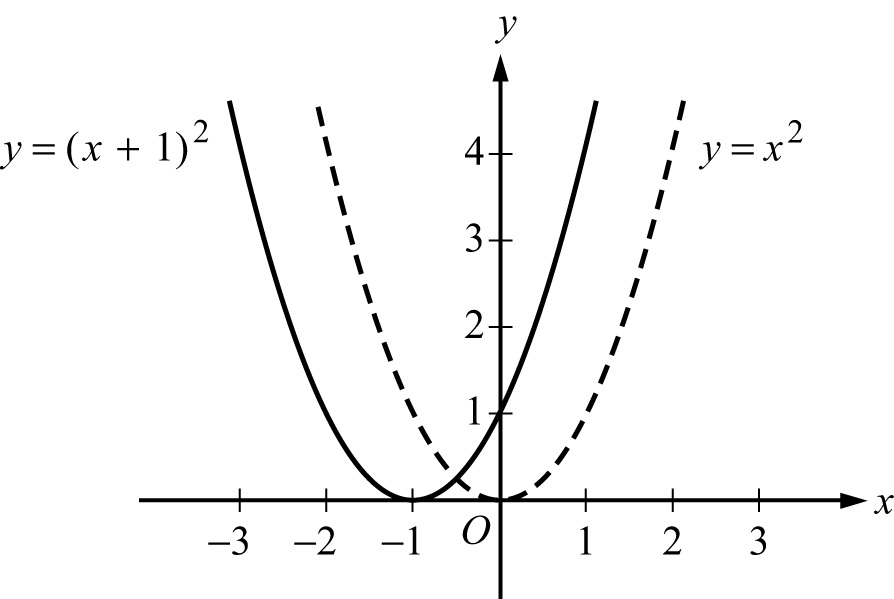
\includegraphics[width=0.5\linewidth]{Shifting_Function2.jpg} 
	\end{figure}
	
\end{frame}
%------------------------------------------------

\subsection{Stretching Functions}
\begin{frame}
	\frametitle{Stretching or Shrinking Functions}
	\begin{theorem}[增大或者缩小开口:函数乘常数项]
		\begin{itemize}
			\item The graph of $ch(x)$ is the graph of $h(x)$ stretched vertically by a factor of c if $c > 1$.
			\item The graph of $ch(x)$ is the graph of $h(x)$ shrunk vertically by a factor of c if $c < 1$.
		\end{itemize}
	\end{theorem}

	\begin{columns}[t] 
		\begin{column}{0.5\textwidth} % Left column width
				\begin{figure}
					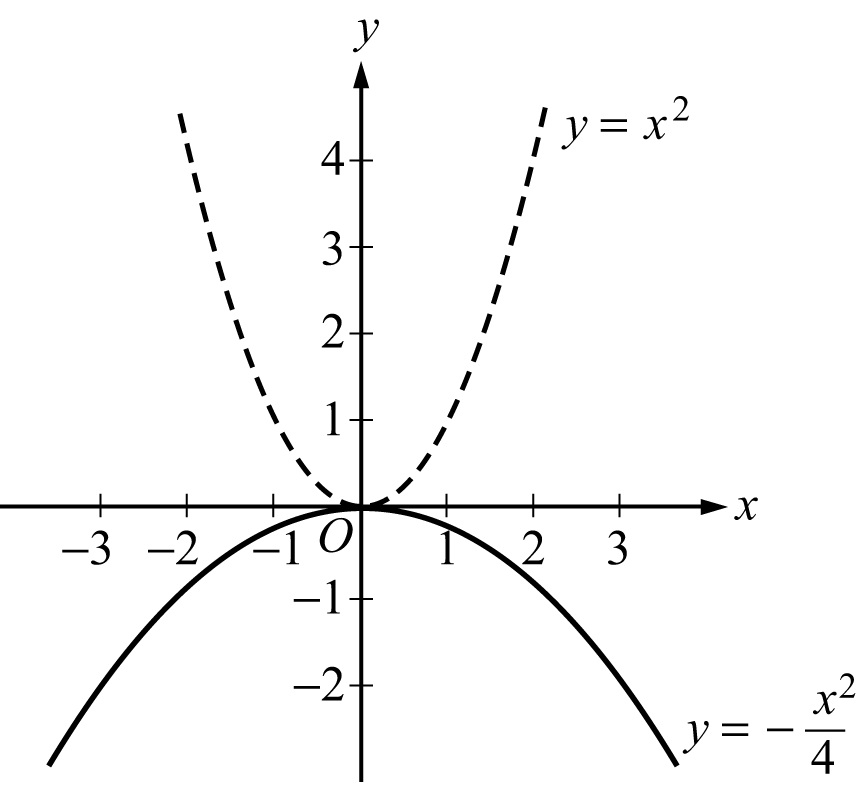
\includegraphics[width=0.6\linewidth]{Shrinking_Functions1.jpg} 
				\end{figure}
		\end{column}
		\begin{column}{0.5\textwidth} % Right column width
			\begin{figure}
					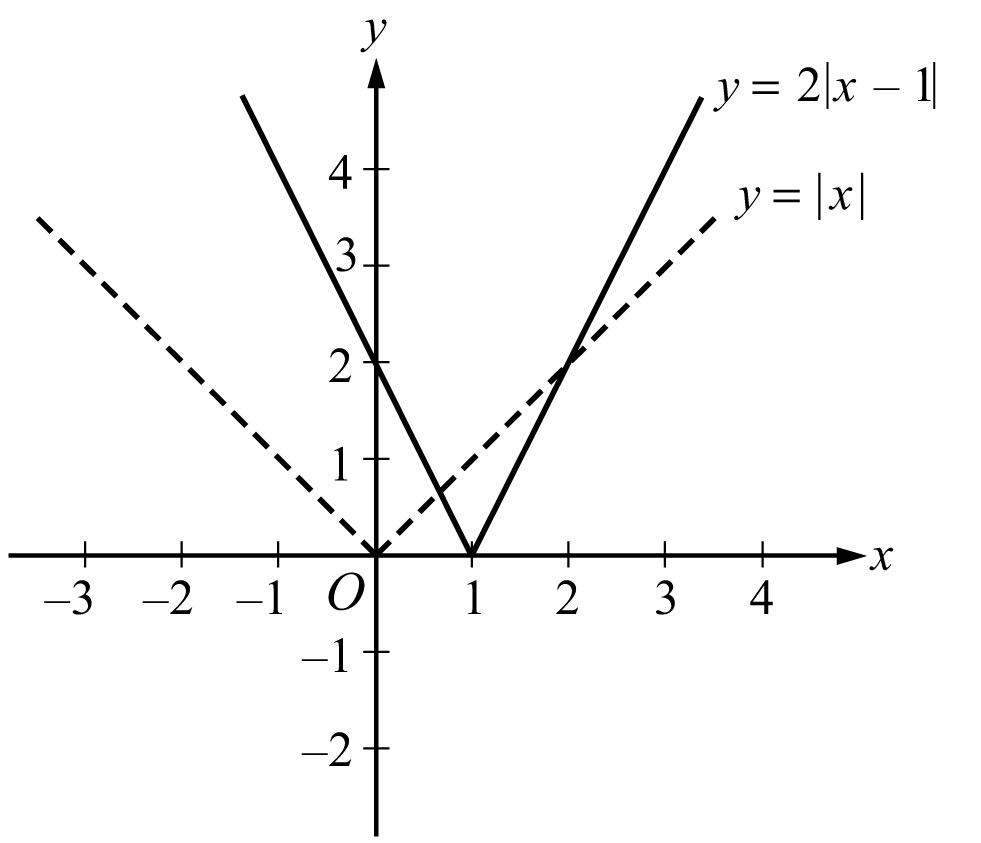
\includegraphics[width=0.6\linewidth]{Shrinking_Shifting_Functions1.jpg} 
			\end{figure}
    \end{column}
	\end{columns}
\end{frame}

%------------------------------------------------

\section{Applications}

%------------------------------------------------

\begin{frame}
\frametitle{Strategy}
{\LARGE Translate from Words to an Arithmetic or Algebraic Representation}
\end{frame}
%------------------------------------------------

\subsection{Average, Mixture, Rate, and Work Problems}

%------------------------------------------------

\begin{frame}
	\frametitle{Average Problems: Have A Try!}
	\framesubtitle{求平均}
	\textbf{og-p375-2.7.4}
	Ellen has received the following scores on 3 exams: 82, 74, and 90. What score will Ellen need to receive on the next exam so that the average (arithmetic mean) score for the 4 exams will be 85 ?
	\pause
	$\frac{82 + 74 + 90 + x}{4} = 85$

	\pause
	Answer: \textbf{94}
\end{frame}

%------------------------------------------------

\begin{frame}
	\frametitle{A Real QR Problem!}
	\framesubtitle{}
	\begin{figure}
		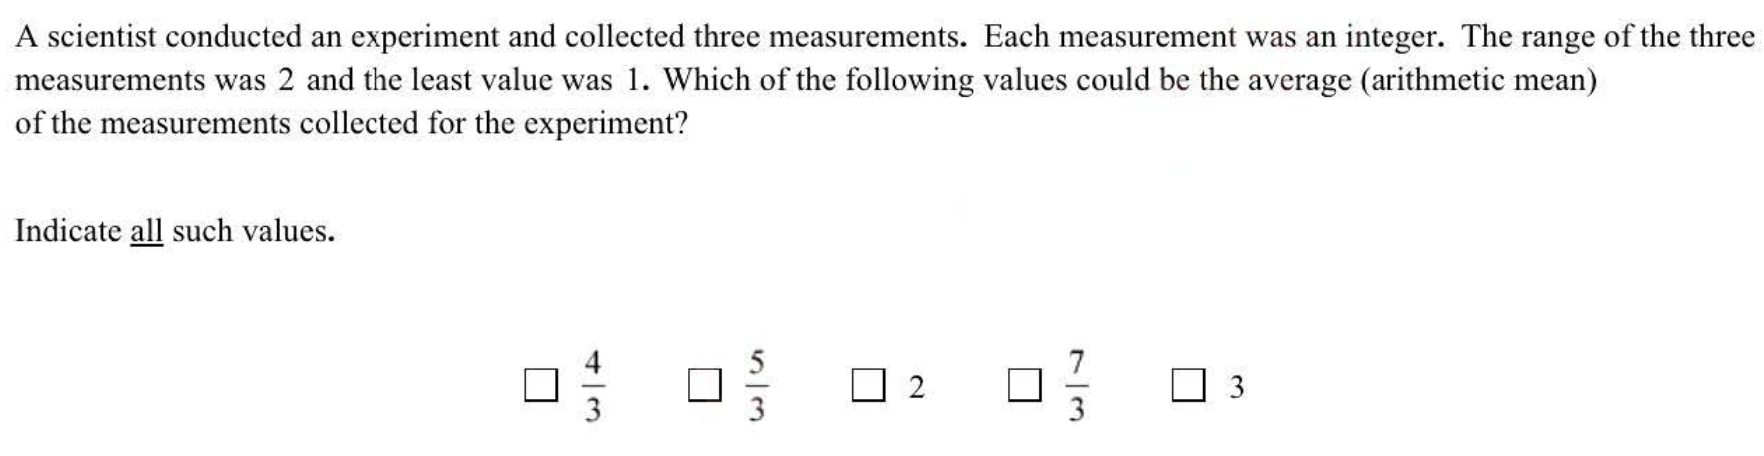
\includegraphics[width=\linewidth]{Average_Example_Question1.png}
		\caption{6-Sec3-13}
	\end{figure}
	\pause
$\because$ The range is 2 and the least value is 1 \\ 
$\therefore$ Two of three integers must be 1 and 3. 
The rest one could be 1, 2, or 3.
$\therefore$ The sum of the measurements could be 5, 6, and 7.\\
\pause
\bigskip
Answer \textbf{BCD: } $\frac{5}{3};2;\frac{7}{3}$
\end{frame}

%------------------------------------------------

\begin{frame}
	\frametitle{Mixture Problems: Have A Try!}
	\framesubtitle{求混合比例}
	\textbf{og-p376-2.7.5}
	A mixture of 12 grams of vinegar and oil is 40 percent vinegar, where all of the measurements are by weight. How many grams of oil must be added to the mixture to produce a new mixture that is only 25 percent vinegar?\\
	\pause
	$\frac{12 \times 0.4}{12 + x} = 25\%$

	\pause
	Answer: \textbf{7.2 grams}
\end{frame}

%------------------------------------------------

\begin{frame}
	\frametitle{Rate Problems: Have A Try!}
	\framesubtitle{求速率}
	\textbf{og-p376-2.7.6}
	In a driving competition, Jeff and Dennis drove the same course at average speeds of 51 miles per hour and 54 miles per hour, respectively. If it took Jeff 40 minutes to drive the course, how long did it take Dennis?\\
	\pause
	\bigskip
	\begin{equation*}
	  \begin{aligned}
	  		&d= r_{J} t_{J} = 51 \unit{mile/\hour} \times \frac{40 \unit{\minute}}{60\unit{\minute / \hour}} = 34 \unit{miles}\\
		    &t_D = \frac{d}{r_d} = \frac{34 \unit{mile}}{54 \unit{mile / \hour}} \times 60\unit{\minute / \hour} \approx 37.8 \unit{\minute}
	  \end{aligned}
	\end{equation*}


	\pause
	\bigskip
	Answer: \textbf{37.8 \unit{mins}}
\end{frame}

%------------------------------------------------

\begin{frame}
	\frametitle{Rate Problems: Have A Try!}
	\framesubtitle{求速度}
	Six machines, each working at the same constant rate, together can complete a certain job in 12 days. How many additional machines, each working at the same constant rate, will be needed to complete the job in 8 days?
	\bigskip
	\pause
	\begin{equation*}
	  \begin{aligned}
	  		&w = x \cdot r \cdot t = 6 \cdot r \cdot 12\\
		    &x\prime = \frac{w}{r\cdot t\prime} = \frac{6 \cdot r \cdot 12}{r \cdot 8} = 9
	  \end{aligned}
	\end{equation*}
\pause 
\alert{Is 9 the final answer?}

	\pause
	\bigskip
	Answer: \textbf{3 Additional Machines}
\end{frame}

%------------------------------------------------

\begin{frame}
	\frametitle{A Real QR Problem!}
	\framesubtitle{}
	\begin{figure}
		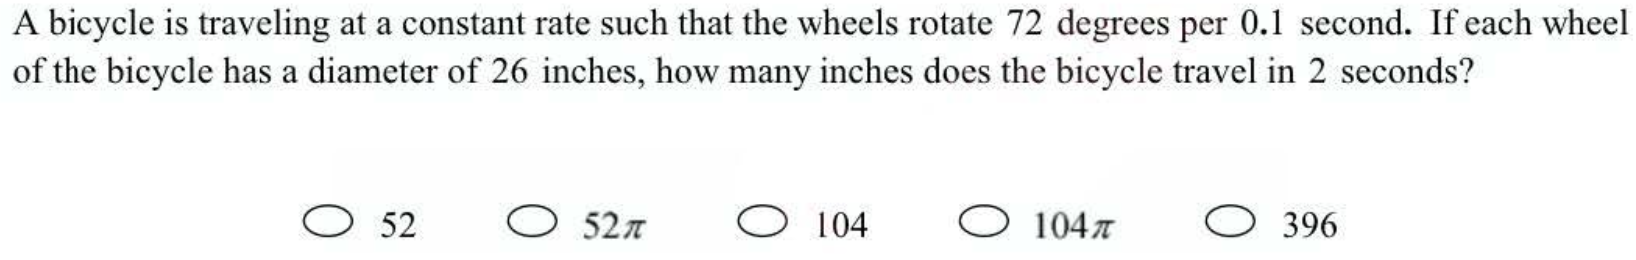
\includegraphics[width=\linewidth]{Rate_Example_Question1.png}
		\caption{7-Sec3-8}
	\end{figure}
	\pause
	\begin{equation*}
	  \begin{aligned}
	  		&degree =  r \cdot t = \frac{\ang{72}}{0.1 \unit{\second}} \cdot 2 \unit{\second} = \ang{1440}\\
		    &circumference = 2 \pi \cdot radius  = 26 \pi \ \unit{inch}\\
		    & distance = \frac{degree}{\ang{360}} \cdot circumference = \frac{\ang{1440}}{\ang{360}} \cdot 26 \pi \ \unit{inch}= 104 \pi \ \unit{inch}
	  \end{aligned}
	\end{equation*}
	\pause
	\bigskip
	Answer \textbf{D: } $104\pi$
\end{frame}

%------------------------------------------------

\begin{frame}
	\frametitle{Work Problems: Have A Try!}
	\framesubtitle{求速率}
	\textbf{og-p377-2.7.7}
	A batch of computer parts consists of n identical parts,
where n is a multiple of 60. Working alone at its constant rate, machine A
takes 3 hours to produce a batch of computer parts. Working alone at its
constant rate, machine B takes 2 hours to produce a batch of computer
parts. How long will it take the two machines, working simultaneously at
their respective constant rates, to produce a batch of computer parts?\\
	\pause
	\bigskip
	\begin{equation*}
	  \begin{aligned}
	  		&r_A = \frac{w}{t_A}= \frac{1}{3} \\
	  		&r_B = \frac{w}{t_B}= \frac{1}{2} \\
		    &t_{A+B} = \frac{w}{r_A + r_B} = \frac{1}{\frac{1}{3}  + \frac{1}{2}} = \frac{6}{5} = 1.2 \unit{\hour}
	  \end{aligned}
	\end{equation*}


	\pause
	\bigskip
	Answer: \textbf{1.2 \unit{\hour}}
\end{frame}

%------------------------------------------------

\subsection{Interest}

\begin{frame}
	\frametitle{Simple Interest v.s. Compound Interest}
	\framesubtitle{单利 \ 复利 }

	\begin{columns}[t] 
		\begin{column}{0.5\textwidth} % Left column width
			\begin{equation*}
			  \begin{aligned}
			  	&Simple\ Interest:\	V =P(1 + \frac{rt}{100})\\
			  	&Compound\ Interest:\	V =P(1 + \frac{r}{100})^t\\
			  \end{aligned}
			\end{equation*}
			\begin{itemize}
				\item P: the principal 本金 
			  \item		r:  the simple annual interest rate of r  percent  年利率
			  \item		t:  t years  时间(年)
			  \item		V:  the value V of the investment at the end of t years  最终金额
			\end{itemize}
		\end{column}

		\begin{column}{0.5\textwidth} % Right column width
			\begin{figure}
				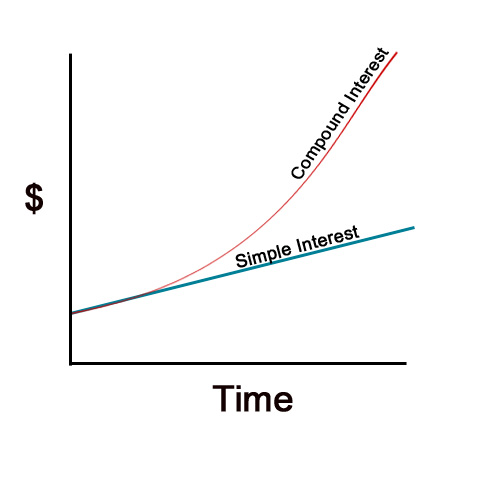
\includegraphics[width=\linewidth]{Simple_Interest_Compound_Interest.jpeg}
				\caption{Compound Interest follow a exponential curve.}
			\end{figure}
    \end{column}
	\end{columns}
\end{frame}

%------------------------------------------------
\begin{frame}
	\frametitle{Compounded Quarterly Or Monthly}
	\framesubtitle{复利的结算周期}

	\begin{columns}[t] 
		\begin{column}{0.5\textwidth} % Left column width
			\begin{equation*}
			  \begin{aligned}
			  	&Compound\ Interest:\\ 	&V =P(1 + \frac{r}{100n})^{nt}\\
			  \end{aligned}
			\end{equation*}
			\begin{itemize}
				\item P: the principal 本金 
			  \item		r:  the simple annual interest rate of r  percent  年利率
			  \item		t:  t years  时间(年)
			  \item		V:  the value V of the investment at the end of t years  最终金额
			  \item n: the times of compounding interest into the principal
			\end{itemize}
		\end{column}

		\begin{column}{0.5\textwidth} % Right column width
			\begin{figure}
				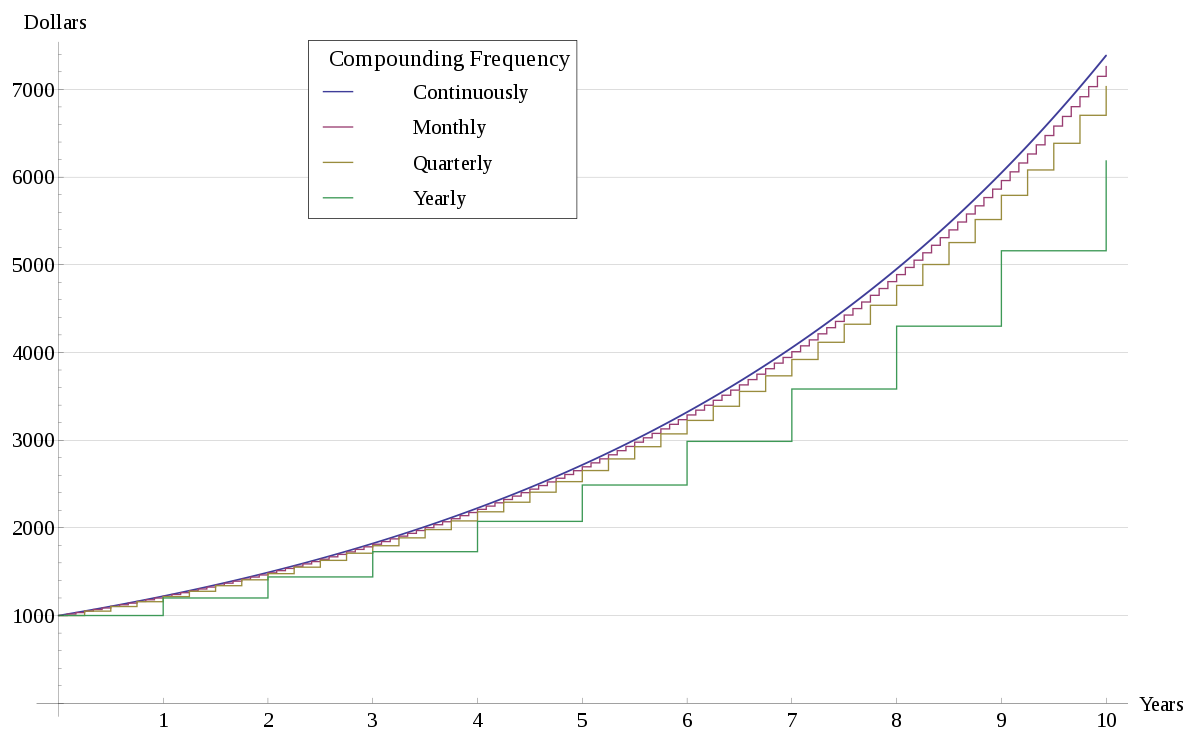
\includegraphics[width=\linewidth]{Compound_Interest_with_Varying_Frequencies.svg.png}
				\caption{compound interest continuously, monthly, quarterly and yearly}
			\end{figure}
    \end{column}
	\end{columns}
\end{frame}

%------------------------------------------------


\begin{frame}
	\frametitle{Interest Problems: Have A Try!}
	\framesubtitle{分清楚单利复利}
	\textbf{og-p379-2.7.10}
If \$ 10,000 is invested at a simple annual interest rate of 6 percent, what is the value of the investment after half a year?
	\bigskip
	\pause
	\begin{equation*}
	  \begin{aligned}
	  		&V =P(1 + \frac{rt}{100})\\
		    &= \$ 10000(1+0.06 (\frac{1}{2}))\\
		    &= \$ 10,300
	  \end{aligned}
	\end{equation*}

	\pause
	\bigskip
	Answer: \textbf{\$ 10,300}
\end{frame}

%------------------------------------------------


\begin{frame}
	\frametitle{Interest Problems: Have A Try!}
	\framesubtitle{注意近似要求}
	\textbf{og-p379-2.7.11}
If an amount P is to be invested at an annual interest rate
of 3.5 percent, compounded annually, what should be the value of P so
that the value of the investment is \$ 1,000 at the end of 3 years? (Give your
answer to the nearest dollar.)
	\bigskip
	\pause
	\begin{equation*}
		\begin{aligned}
					V &=P(1 + \frac{r}{100})^t \\
					  &= P(1+ 0.035)^3\\
					  &= \$ 1000 \\
			    P &= \frac{\$ 1000 }{(1+ 0.035)^3}\\
			      &\approx \$ 902 					 
		\end{aligned}		
	\end{equation*}
	\pause
	\bigskip
	Answer: \textbf{\$ 902 }
\end{frame}

%------------------------------------------------


\begin{frame}
	\frametitle{A Real QR Problem!}
	\framesubtitle{}
	\begin{figure}
		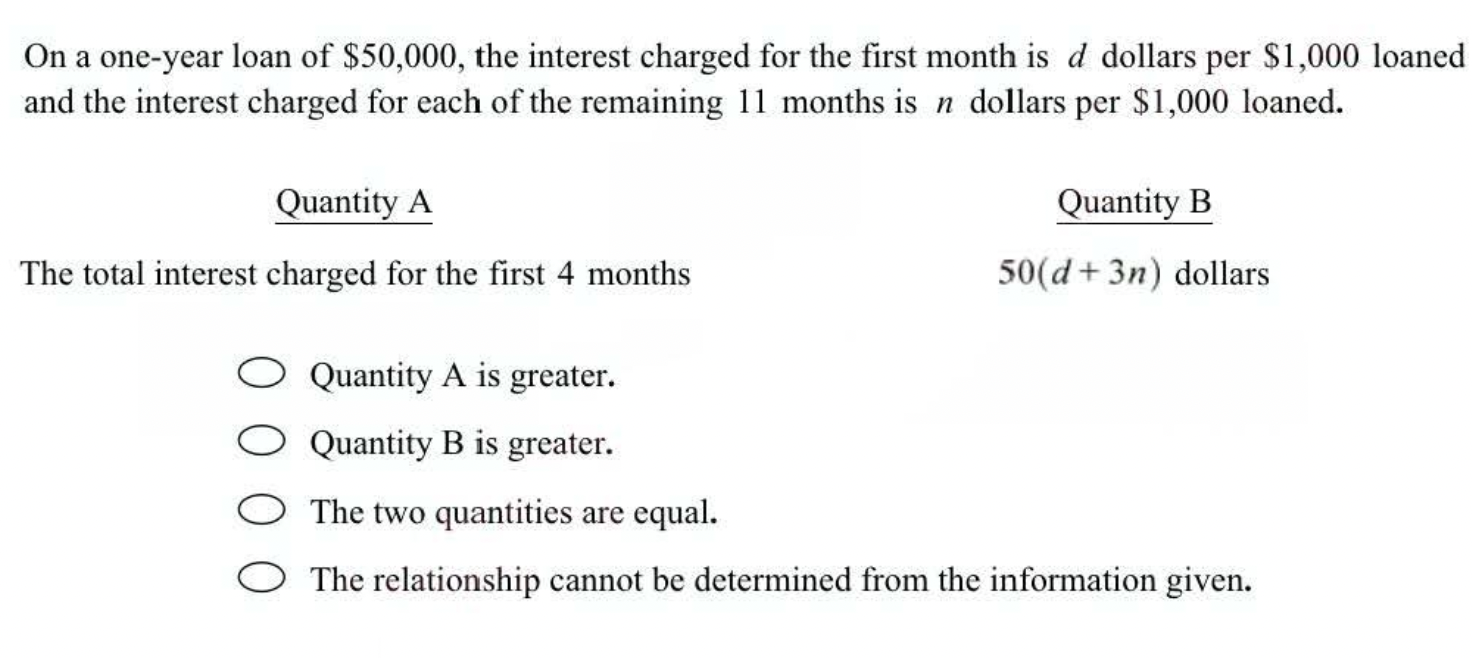
\includegraphics[width=\linewidth]{Interest_Example_Question1.png}
		\caption{4-Sec1-6}
	\end{figure}
	\pause
\alert{Money Loaned!!}\\
	\bigskip
	Answer \textbf{C: } The two quantities are equal
\end{frame}

%------------------------------------------------

\begin{frame}
	\frametitle{A Real QR Problem!}
	\framesubtitle{}
	\begin{figure}
		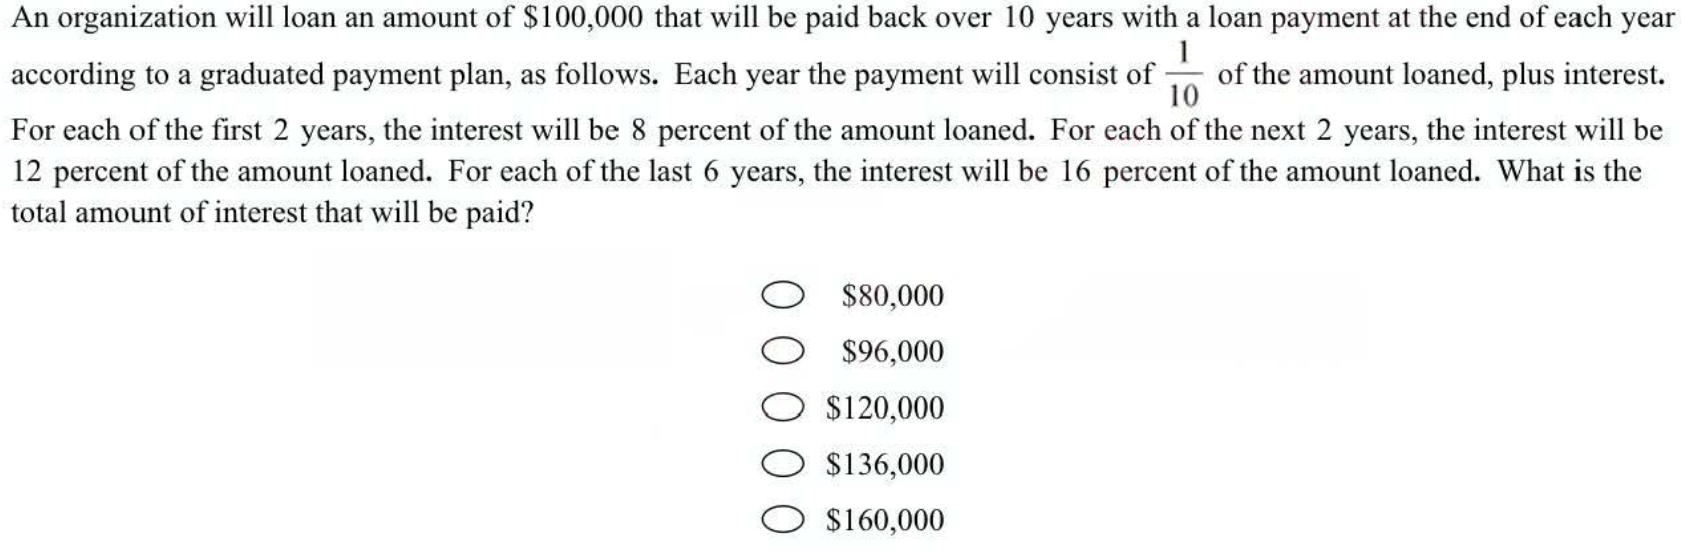
\includegraphics[width=\linewidth]{Interest_Example_Question2.png}
		\caption{4-Sec3-11}
	\end{figure}
	\pause
	$(0.08 \times 2 + 0.12 \times 2 + 0.16 \times 6) \times \$100,000= \$136,000$\\
\alert{Amount Loaned}\\
	\bigskip
	Answer \textbf{D: } \$136,000
\end{frame}


%----------------------------------------------------------------------------------------
%	CLOSING SLIDE
%----------------------------------------------------------------------------------------

\begin{frame}[plain] % The optional argument 'plain' hides the headline and footline
	\begin{center}
		{\Huge 1 Min Break}
		\bigskip\bigskip % Vertical whitespace
		
		{\LARGE Questions? Comments?}
	\end{center}
\end{frame}

%----------------------------------------------------------------------------------------

\end{document} 